% vim: spelllang=fr

\documentclass[../main.tex]{subfiles}
\graphicspath{{\subfix{../Figures/Chap2/}}}
\begin{document}

\begin{itshape}
Ce deuxième chapitre porte de l'approche directe consistant en l'application d'un algorithme de détection et de suivi des cyclones tropicaux dans les modèles
comme façon de caractériser l'activité cyclonique simulée, ainsi que la façon dont les modèles représentent ces phénomènes. Un cas d'étude est présenté via
l'application du schéma de détection du CNRM à la réanalyse ERA5.
\end{itshape}

\minitoc\newpage
%--------------------------------------

\section{Introduction}\label{sec:intro_chap2}

Les algorithmes de détection et de suivi des HTV dans les modèles consistent à identifier les points de grille qui satisfont des critères thermiques ou
dynamiques associés à un cyclone tropical. Le \cref{chap:chapitre_1}, en particulier la \cref{sec:intro_tracking}, met en évidence la sensibilité de l'activité
cyclonique mesurée au choix de la méthode de détection et montre que ce choix peut aboutir à des conclusions différentes quant au signe du changement dans des
expériences à climat plus chaud. En effet, si tous les traqueurs de TC partagent le même objectif, les méthodologies utilisées dans la littérature présentent
néanmoins une très grande diversité. Les premiers schémas de détection étaient basés uniquement sur la MSLP et la vitesse des vents
\parencite{bengtsson_simulation_1982,broccoli_can_1990}, tandis que \cite{haarsma_tropical_1993,bengtsson_hurricanetype_1995} ajoutèrent à cela des critères sur
la vorticité ainsi qu'un diagnostique sur la présence d'un cœur chaud, dans l'optique de discriminer les perturbations tropicales de leurs homologues
extratropicales. \cite{wu_gcm_1992} utilisent des critères supplémentaires conçus pour discriminer les perturbations tropicales sèches via un seuil d'humidité
relative, les perturbations équatoriales d'est en interdisant le vent d'est à \hPa{950} au point situé à \ang{4.5} au nord et au sud du cyclone, ainsi que les
perturbations barocliniques en bornant la vitesse du vent d'ouest à \hPa{200} au dessus du centre du cyclone à \ms{5}. Dans \cite{bengtsson_hurricanetype_1995},
la méthodologie de détection introduit des tests de structure verticale du système, aussi bien sur le profil de vent que de température. En effet, après avoir
identifié un centre cyclonique à travers la vorticité, pression minimum locale et vitesse du vent maximale dans une boîte autour du système, il s'agit alors de
s'assurer de la présence d'une anomalie de température sur l'ensemble de la troposphère, par rapport à la moyenne prise dans cette boîte, puis de s'assurer
également que l'anomalie à la tropopause est supérieure que celle à la couche limite. Un test similaire est réalisé sur le profil vertical de vent, en imposant
que le vent moyen à \hPa{850} supérieur à la moyenne du niveau à \hPa{300}, toujours dans la boîte centrée. Beaucoup d'algorithmes de détection reprennent cette
méthodologie, avec quelques variantes et spécificités. Une grande quantité de méthodologies et de seuils de détection sont décrits dans
\cite{walsh_objectively_2007} ainsi que dans \cite[][Annexe B]{ullrich_tempestextremes_2017}, schémas dans lesquels la définition d'un TC et les valeurs
numériques utilisées pour les divers seuils de détection sont souvent choisis de telle sorte à reproduire au mieux la climatologie observée
\parencite{walsh_objectively_2007,tory_development_2013}.

Parmi les traqueurs possédant des particularités remarquables, le plus communément utilisé est sans aucun doute le schéma de détection TRACK
\parencite{hodges_how_2017}. Ce dernier a la particularité de systématiquement interpoler les champs du modèle à une basse résolution (T63, soit \km{210}),
avant d'appliquer un schéma de détection basé exclusivement sur la vorticité. Cela permettrait de s'affranchir de la sensibilité de la méthode de détection à la
résolution du modèle. Cet algorithme a cependant tendance à détecter une quantité parfois anormalement élevée de systèmes (voir \cref{fig:NTC_HighResMIP_TRACK}
par rapport à la \cref{fig:NTC_HighResMIP}), et est alors particulièrement sujet à la détection de faux-positifs \parencite{bourdin_intercomparison_2022}. La
problématique que TRACK vise à solutionner est néanmoins bien réelle. La résolution du modèle impacte la représentation des TC dans les modèles ce qui implique
que les traqueurs doivent souvent être ajustés pour chaque résolution. Une autre alternative se trouve dans \cite{camargo_improving_2002} où les auteurs ont
proposé une méthode de détection de HTV dont les seuils pour chacune des variables sont déterminées à partir de la climatologie du modèle. Spécifiquement, ces
derniers s'expriment sous la forme $\alpha \sigma + \beta$, où $\alpha$ et $\beta$ sont issues de la climatologie globale du modèle, et où $\sigma$ représente
l'écart type de la variable à l'échelle de chaque bassin océanique. Le schéma de détection de \cite{camargo_improving_2002} possdède par ailleurs la
fonctionnalité intéressante visant à compléter en amont et en aval les trajectoires détectées. Pour ce faire les contraintes sur les paramètres de détection
sont relâchées et le traqueur cherche alors à suivre un signal de vorticité jusqu'à que cette dernière tombe en dessous d'un certain seuil prévu à cet effet. Ce
processus de relaxation permet de prolonger les trajectoires détectées, qui sont sinon souvent courtes, et permet notamment d'éviter de scinder en deux
trajectoires un système dont une ou plusieurs variables seraient temporairement passées en dessous des seuils de détection. La méthode des seuils de détection
climato-statistiques de \cite{camargo_improving_2002} n'est cependant pas largement répandue, possiblement parce que d'une part, les valeurs $\alpha$ et $\beta$
pour chacune des variables se déterminent par les densités de probabilités bivariées dont l'estimation est complexe et laborieuse, et d'autre part parce que
cette approche représente un paradigme très différent des traqueurs mentionnés précédemment. En effet, les traqueurs à seuils fixes visent à appliquer un schéma
de fonctionnement conceptuel d'un cyclone tropical au modèle, ce qui permet ensuite d'établir dans quelle mesure le modèle est capable de simuler des systèmes
réalistes, là où la méthode de \cite{camargo_improving_2002} cherche au contraire à s'affranchir des biais intrinsèques au modèle, en considérant que les TC
constituent dans tous les cas les extrêmes des distribution des variables d'intérêt. Il faut cependant noter que si les traqueurs à seuils absolus permettent
d'évaluer des biais de représentation des TC, ils ont également le défaut de rendre indiscernables les erreurs issues du modèle de celles issues du schéma de
détection lui-même, contribuant aux incertitudes quant à l'évolution future de la fréquence des cyclones tropicaux dans un climat plus chaud mentionnées dans le
\cref{chap:chapitre_1}, \cref{sec:intro_tracking}. Ces deux catégories de traqueurs ont donc chacun leurs avantages et leurs inconvénients.

Ainsi, pour espérer comprendre la divergence entre les projections issues de l'approche directe et indirecte, il est nécessaire de pouvoir évaluer
quantitativement la performance d'un schéma de détection et de suivi objectif de cyclones tropicaux. Une solution consiste à appliquer un schéma de détection à
une simulation dont les trajectoires sont à priori connues d'avance, en utilisant une réanalyse atmosphérique. Les réanalyses combinent des prévisions
météorologiques à court terme avec des observations passées via un modèle et un schéma d'assimilation de données ---~permettant de corriger la trajectoire du
modèle lorsque ce dernier s'éloigne de l'état connu de l'atmosphère~--- invariants sur toute la période d'analyse. Une réanalyse offre donc une vision globale
de l'atmosphère qui est cohérente dans le temps et l'espace et qui intègre au mieux l'ensemble des observations qui y sont intégrées, si bien que le produit
final constitue une excellente estimation de l'état passé de l'atmosphère sur toute la période considérée. Il en résulte que la plupart ---~sinon
l'intégralité~--- des cyclones tropicaux observés et référencés dans la base données IBTrACS, introduite dans le \cref{chap:chapitre_1},
\cref{sec:observations}, sont à priori présents dans une réanalyse.

Dans ce chapitre, on considère le schéma de détection du CNRM, à l'origine conçu pour suivre les dépressions de moyennes latitudes par
\cite{ayrault_nouvelle_2000} puis adapté aux cyclones tropicaux dans \cite{chauvin_response_2006}, et utilisé à cette fin par
\cite{daloz_impact_2012,chauvin_atlantic_2017,chauvin_future_2020,cattiaux_projected_2020}. Le modèle conceptuel du fonctionnement d'un TC implémanté dans le
traqueur du CNRM est basé sur \cite{bengtsson_hurricanetype_1995}, avec la particularité de considérer deux disques concentriques, dont les rayons sont évalués
dynamiquement à chaque pas de temps, plutôt qu'une boîte fixe pour discriminer les HTV de leur environnement, et intègre également le processus de relaxation de
\cite{camargo_improving_2002}. Des descriptions détaillées du fonctionnement de cet algorithme sont disponibles dans \cite{chauvin_response_2006}, ainsi que
dans la \cref{sec:papier_data_methods}. Spécifiquement, le traqueur du CNRM est appliqué à la réanalyse ERA5 \parencite{hersbach_era5_2020}. En effet, ERA5 est
la dernière en date du CEPMMT et est la première réanalyse mondiale à atteindre une résolution horizontale de \km{31}, ici interpolée sur une grille à
\ang{0.25}. Elle assimile des données issues de plus d'une vingtaine de satellites d'observations météorologiques, totalisant \num{54} instruments. Aux données
satellitaires s'ajoutent les observations \textit{in-situ} composées de stations au sol, bouées instrumentées, navires marins, radiosondages, radars et avions
de reconnaissance. De par sa résolution inédite et la grande diversité des sources observations qui y sont assimilées, ERA5 constitue donc le choix idéal pour
évaluer la capacité du traqueur à détecter les HTV. Dans la \cref{sec:eval_tracker_ERA5}, les performances du traqueur du CNRM ainsi que sa sensibilité à ses
divers seuils de détection sont évaluées sur ERA5, en termes de probabilité de détection (\textit{Probability of Detection}, POD) et de taux de fausses alarmes
(\textit{False Alarm Rate}, FAR). La capacité d'ERA5 à représenter les TC est également évaluée, via une analyse de leurs caractéristiques en termes
d'intensité, de cycle de vie et également via l'étude de leur profiles verticaux. Ces travaux sont présentés par la publication scientifique dont ils ont fait
l'objet \parencite{dulac_assessing_2023}. Un article complémentaire compare les tracks issues de quatre schémas de détection appliqués à ERA5, dont celui du
CNRM \parencite{bourdin_intercomparison_2022}. Enfin, la \cref{sec:complements_papier} présente des considérations sur le filtrage de systèmes de moyennes
latitudes ---~source de biais important dans les schémas de détection de TC~--- et introduit trois métriques visant à évaluer la ressemblance des trajectoires
détectées dans ERA5 avec les trajectoires historiques.

\section{Évaluation du traqueur CNRM sur ERA5 par rapport à IBTrACS}\label{sec:eval_tracker_ERA5}

\subsection{Résumé de l'article}

La réanalyse ERA5 du Centre européen pour les prévisions météorologiques à moyen terme est la première réanalyse mondiale à atteindre une résolution horizontale
de \km{31} et offre donc une occasion unique d'étudier les cyclones tropicaux, et en particulier les champs 3D associés aux TC historiques. A cette fin, un
algorithme de détection et de suivi des TC spécialement calibré pour ce jeu de données est appliqué sur ERA5 ainsi qu'un algorithme d'appariement des
trajectoires conçu pour associer les trajectoires détectées avec celles issues de la base de données IBTrACS dans le but d'évaluer la capacité de la réanalyse à
représenter les cyclones tropicaux Après optimisation du schéma de suivi et l'application d'une technique de filtrage dynamique des systèmes de moyennes
latitudes, il est montré que la majorité des TC d'IBTrACS sont détectés dans ERA5 et que le nombre de fausses alarmes reste raisonnablement bas dans la plupart
des régions. En comparant les trajectoires détectées dans ERA5 avec leurs équivalents IBTrACS, on constate que l'intensité des TC est encore fortement
sous-estimée dans la réanalyse, mais que la distribution de la pression minimale au niveau de la mer est mieux représentée que la vitesse maximale du vent. Par
ailleurs, la comparaison entre les cycles de vie des deux jeux de données met en évidence des différences essentielles entre ERA5 et les best tracks, avec en
particulier un retard avec lequel les TC d'ERA5 atteignent leur pic d'intensité par rapport à IBTrACS, délai qui augmente de manière significative pour les
cyclones les plus forts. Enfin, les structures verticales des TC dans la réanalyse sont analysées et révèlent une intensification nette jusqu'à la catégorie 3
sur l'échelle de Saffir-Simpson, au delà de quoi les différences sont peu discernables.

La version publiée de \cite{dulac_assessing_2023} est présentée dans la \cref{sec:papier} ci-après, avec la permission de l'éditeur \textit{Springer Nature}.

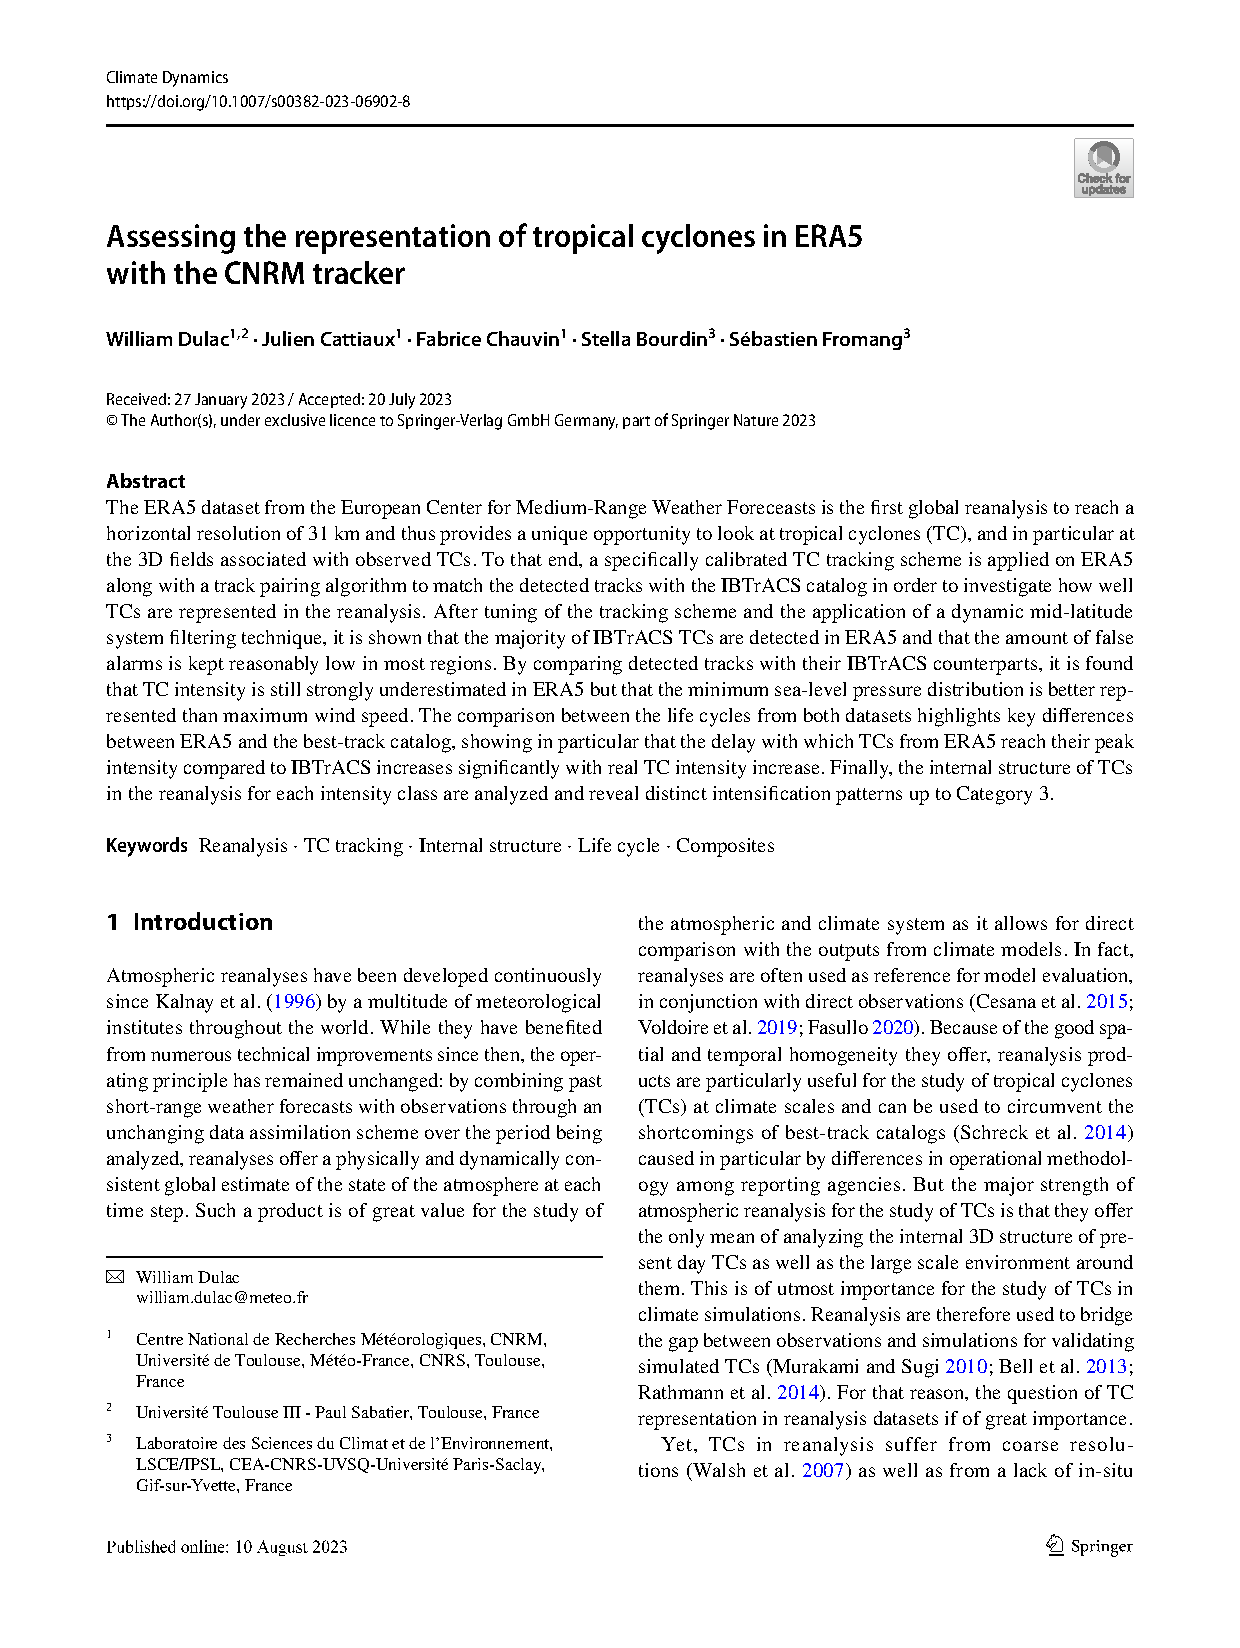
\includepdf[pages=-,pagecommand={\thispagestyle{plain}},offset=5mm 0mm,scale=1,addtotoc=
    {1,subsection,1,Article Climate Dynamics,sec:papier,
     1,subsubsection,2,Introduction,sec:papier_intro,
     2,subsubsection,2,Données et Méthodes,sec:papier_data_methods,
     4,subsubsection,2,Résultats,sec:papier_results,
     10,subsubsection,2,Discussion et conclusion,sec:papier:discussion,
     12,subsubsection,2,Annexe A: Optimisation du traqueur pour ERA5,sec:papier_appendix_A}]{\subfix{../include/dulac2023.pdf}}
%
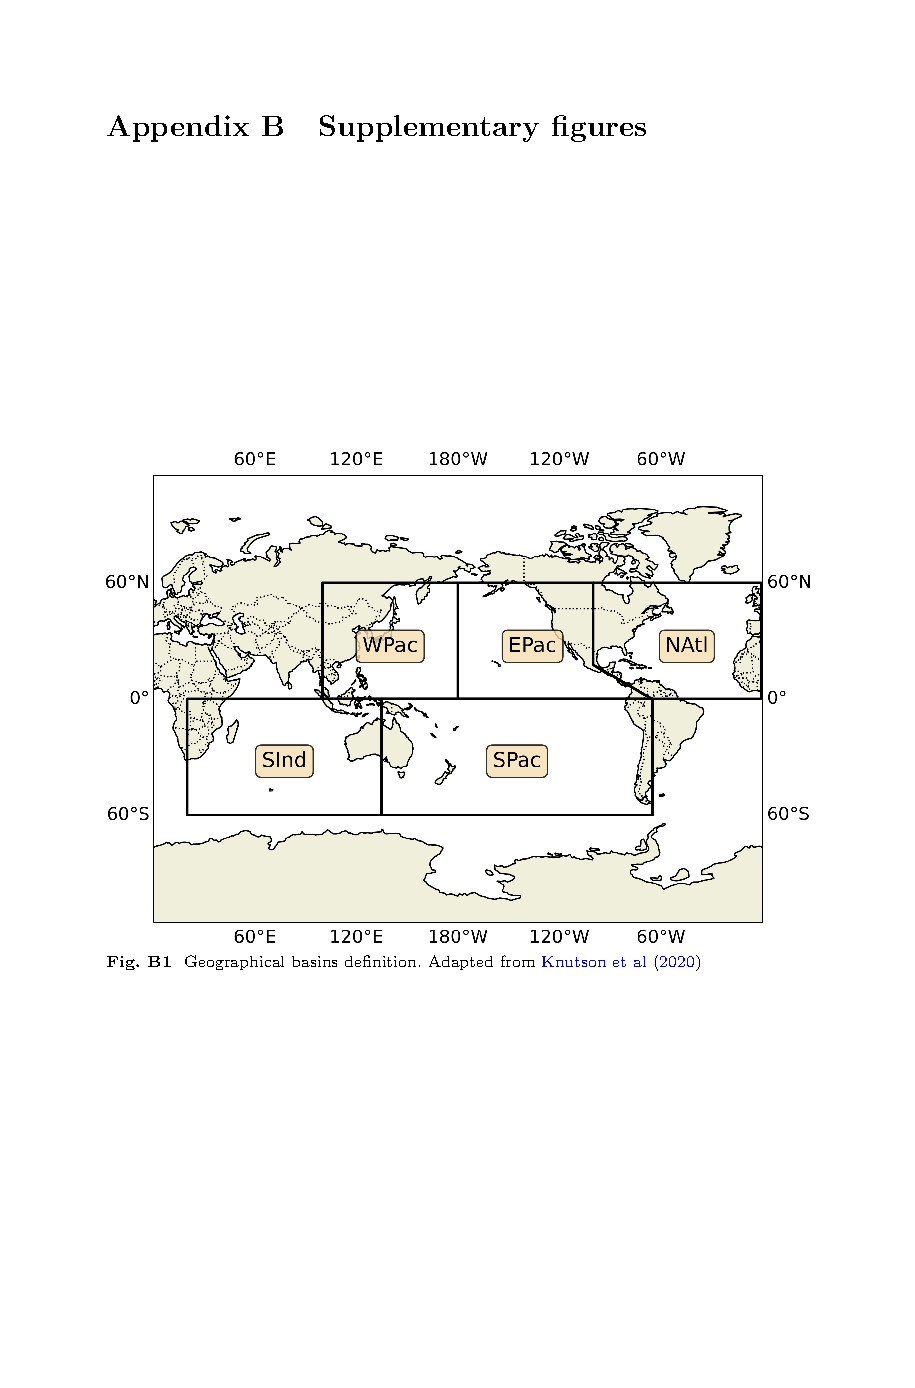
\includepdf[pages=-,pagecommand={\thispagestyle{plain}},offset=5mm 0mm,addtotoc=
{1,subsubsection,2,Annexe B: Figures supplémentaires,sec:papier_appendix_B}]{\subfix{../include/appendix_B_empty.pdf}}

\section{Compléments}\label{sec:complements_papier}

\subsection{Filtrage des systèmes de moyennes latitudes}\label{sec:filtrage_mid_latitudes}

\subsection*{Introduction}

La détection des cyclones tropicaux dans la réanalyse ERA5 et l'appariement de ces derniers avec le catalogue des best tracks, tel que pratiqué dans
\cite{dulac_assessing_2023} et présenté dans la \cref{sec:papier}, révèle une quantité significative de systèmes identifiés \textquote{faux positifs} par
l'algorithme d'appariement. Ces cas correspondent à des systèmes détectés dans la réanalyse mais pour lesquels aucune correspondance n'est identifiée dans
IBTrACS. Dans \cite{dulac_assessing_2023}, le taux de faux-positivité intégré sur la période \num{1981}~--~\num{2019} et sur les cinq bassins océaniques
d'intérêt s'élève à \prct{24} (\cref{sec:papier_results}). Lorsque le filtre appliqué en post-traitement et basé sur le paramètre $V_U^T$ de l'espace des phases
de \cite{hart_cyclone_2003} est désactivé, cette quantité vaut alors \prct{60}. Une valeur $V_U^T < 0$, où $V_U^T$ est défini comme le gradient vertical entre
\hPa{600} et \hPa{300} de la perturbation de hauteur géopotentielle maximale dans un rayon de \km{500} centré sur le cyclone, est indicatif de la présence d'un
vent thermique (induit par un gradient de température) plus fort à \hPa{600} qu'à \hPa{300}. Ce paramètre permet alors de discriminer les cyclones tropicaux à
cœur chaud des tempêtes extratropicales qui présentent souvent un cœur froid. Si ce filtre est si efficace, c'est en effet parce que la grande majorité des
faux-positifs détectés par le traqueur dans ERA5 sont des systèmes de moyenne latitudes, comme en atteste la \cref{fig:lat_density} qui présente pour les faux
positifs sans ce filtre un mode principal centré sur \ang{50}N et S pour les deux hémisphères respectifs. L'activation du filtre $V_U^T$
(\cref{fig:lat_density}.b) inverse la tendance dans l'hémisphère sud, puisque le mode secondaire situé juste en dessous de \ang{25}S devient le mode principal,
et l'écart entre les deux modes dans l'hémisphère nord se réduit lorsque le filtre est activé. La quantité de ces derniers est en partie un effet secondaire de
l'optimisation des seuils de détection dans le but de maximiser la probabilité de détection, présentée dans la \cref{sec:papier_appendix_A}, mais les faux
positifs du jeu de trajectoires obtenu avant optimisation, avec des seuils plus restrictifs, sont aussi largement constitués de systèmes extratropicaux.

\begin{figure}[tb]
    \centering
    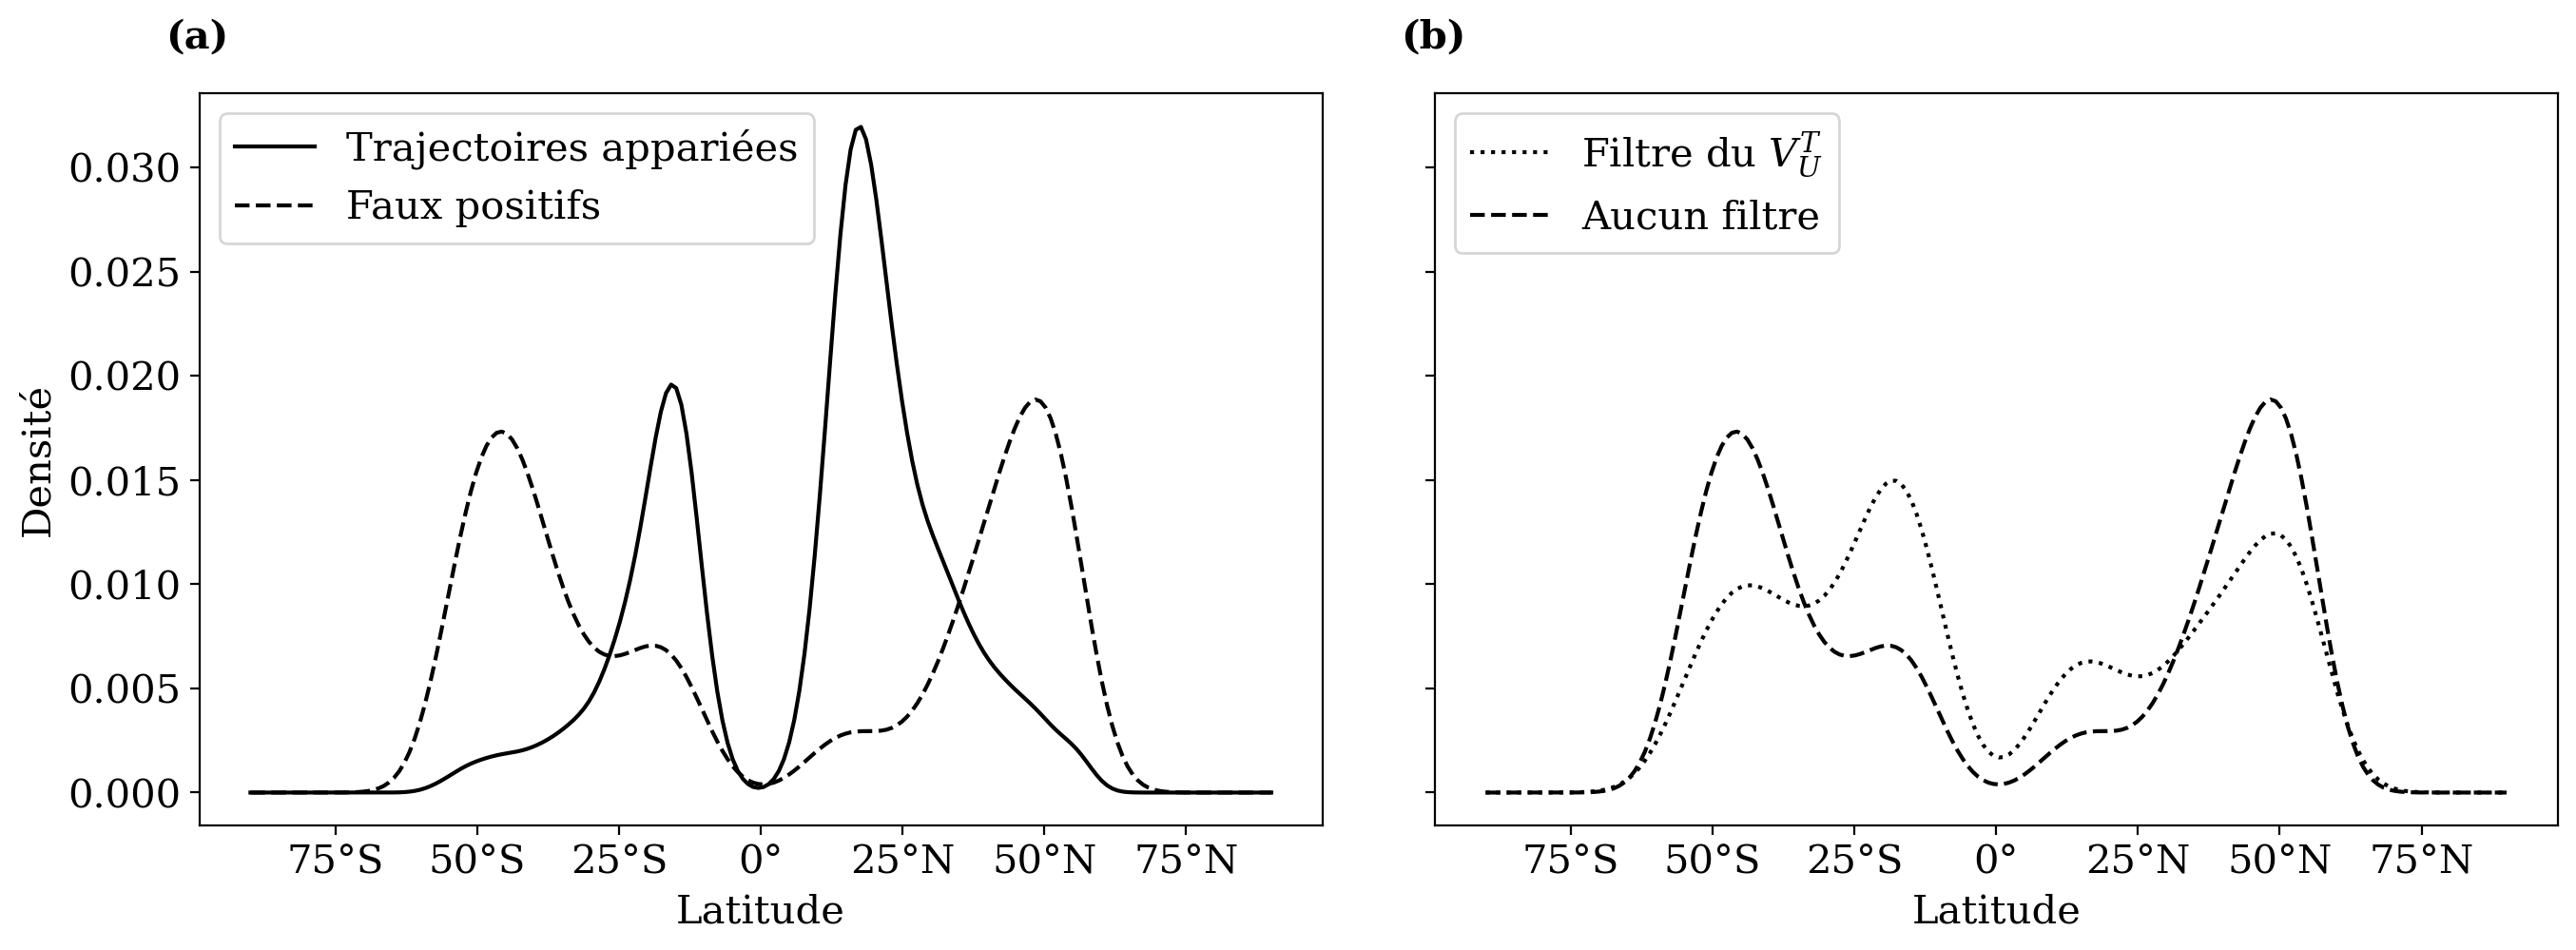
\includegraphics[width=\textwidth]{genesis_lat_density_opti_w_wo_filter.png}
    \caption{(a) Densités de probabilités estimées par noyau gaussien de la latitude d'origine d'une trajectoire ERA5 selon si elle est appariée avec IBTrACS
    (trait plein) ou identifée comme faux positif (tirets), réalisées sur les trajectoires issues du schéma de détection optimisé lorsque le filtre basé sur
    le paramètre $V_U^T$ est désactivé. (b) Densités de probabilités de la latitude d'origine des faux positifs : sans le filtre $V_U^T$ (tirets), identique
    à l'encadré (a), et avec le filtre $V_U^T$ (pointillés).}
    \label{fig:lat_density}
\end{figure}

La discrimination des cyclones tropicaux des autres systèmes météorologiques tourbillonnaires constitue la difficulté principale de la détection objective de TC
dans les modèles, et est la raison pour laquelle beaucoup de traqueurs, notamment ceux basés sur la méthodologie de \cite{bengtsson_hurricanetype_1995},
fournissent une description si détaillée d'un TC à travers les diverses conditions et seuils à respecter, à l'instar du traqueur du CNRM. Force est de constater
que ce n'est cependant pas suffisant, si bien que d'autres stratégies sont parfois employées. La solution la plus simple consiste à définir une contrainte en
latitude. Une telle limite est parfois fixée à \ang{30} \parencite{bengtsson_simulation_1982,broccoli_can_1990,mcdonald_tropical_2005}, ou encore entre \ang{40}
et \ang{45} \parencite{wu_gcm_1992,tsutsui_simulated_1996,tsutsui_implications_2002,oouchi_tropical_2006,zarzycki_multidecadal_2014}. Définir une limite fixe en
latitude pose toutefois problème lorsqu'il s'agit de chercher à détecter les cyclones tropicaux dans des simulations à climat plus chaud, étant donné
l'expansion des tropiques \parencite{lucas_expanding_2014,staten_reexamining_2018} et le décalage vers les pôles de l'activité cyclonique
\parencite{kossin_poleward_2014,knutson_tropical_2020}. Ainsi, un filtre des systèmes de moyennes latitudes pour un schéma de détection ayant vocation à être
appliqué à des simulation de réchauffement climatique se doit de pouvoir s'adapter à un climat altéré, et donc d'être un filtre dynamique.

Dans cette section, nous considérons des filtres alternatifs au $V_U^T$ dans le but d'expliquer les raisons pour lesquelles c'est ce dernier qui a été choisi
dans \cite{dulac_assessing_2023}. Une attention particulière est portée à une solution consistant en l'utilisation de la latitude du maximum de gradient
méridional de hauteur géopotentielle à \hPa{200}. Le parallèle est fait avec la méthode employée dans \cite{bourdin_intercomparison_2022} qui utilise la limite
équatoriale du jet subtropical comme limite méridionale.

\subsubsection*{Filtre du gradient de hauteur géopotentielle à \hPa{200}}

Les courants jet stratosphériques, causés par le gradient de température entre les pôles et l'équateur, apportent du cisaillement qui affaiblissent les cyclones
tropicaux jusqu'à leur faire perdre leurs caractéristiques tropicales et peuvent ensuite transitionner vers l'état de cyclone extratropical. Ces courants sont
liés au gradient de géopotentiel par la relation du vent thermique si bien que la hauteur géopotentielle à \hPa{200}, $Z_{200}$, s'effondre dans les moyennes
latitudes. Cela laisse alors apparaître la perspective d'utilisation de la limite en latitude formée par le maximum de $\partial Z_{200} / \phi$, évalué à
chaque longitude, comme filtre des systèmes de moyennes latitudes. La \cref{fig:ophelia_z200} illustre l'intérêt d'utiliser cette grandeur à travers l'exemple
du cyclone Ophelia de la saison cyclonique 2017, tel que détecté dans la réanalyse ERA5. Si ce cyclone a terminé sa transition extratropicale le 16 Octobre à
00:00, à \km{270} du cap Mizen l'extrémité sud de l'Irlande, correspondant au point situé entre \ang{45} et \ang{50}N sur la \cref{fig:ophelia_z200}, cet
exemple montre néanmoins que ce système a avancé vers le nord dans un méandre de géopotentiel, et est resté en dessous de la latitude du gradient maximal
jusqu'à l'Écosse, formant une trajectoire détectée à laquelle ne manque que trois échéances par rapport à la best track.

\begin{figure}[htpb]
    \centering
    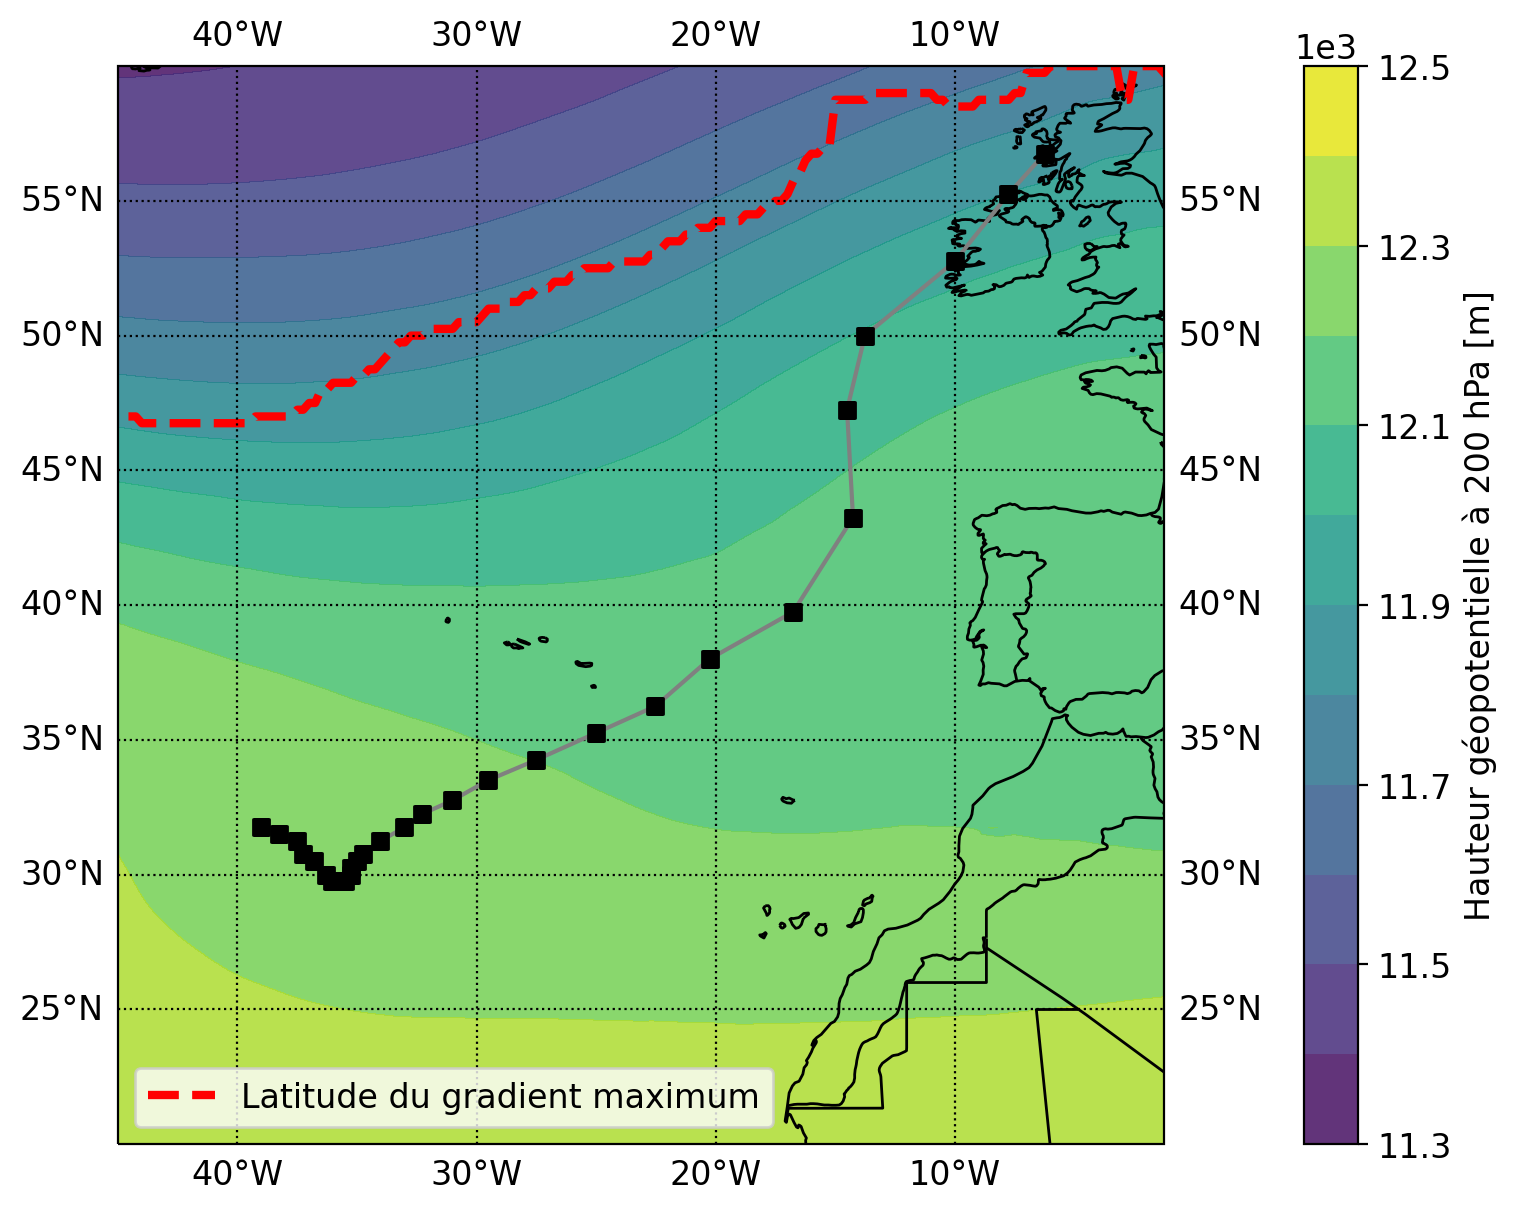
\includegraphics[width=0.7\textwidth]{ophelia_geopdy_mean_geopt.png}
    \caption{Trajectoire détectée dans ERA5 du cyclone Ophelia de la saison cyclonique 2017 sur fond du champ de hauteur géopotentielle à \hPa{200} moyenné
    entre le 10 Octobre 2017 à 06:00 et le 17 Octobre à 00:00, correspondant respectivement à la première et dernière échéance détectée du système. Le tracé
    rouge correspond à la latitude du maximum de gradient méridional du champ présenté.}
    \label{fig:ophelia_z200}
\end{figure}

L'usage du gradient de $Z_{200}$ comme limite méridionale présente par ailleurs l'intérêt d'évoluer de manière saisonnière. C'est ce que montre la
\cref{fig:geopdy_clim} avec la climatologie mensuelle de la latitude du maximum de $\partial Z_{200} / \partial \phi$ sur la période \num{1980}~--~\num{2020},
sous la forme d'un diagramme de Hovmöller. L'encadré (a) de la \cref{fig:geopdy_clim}, correspondant à l'hémisphère nord, montre par exemple que cette limite
méridionale tend à se déplacer vers le pôle durant la saison estivale, en particulier sur l'océan Atlantique, mais aussi sur l'ensemble de l'océan Pacifique,
régions sur lesquelles la moyenne sur le mois d'Août est située au delà de \ang{50}. Inversement, la moyenne mensuelle descend à \ang{39}N au cœur de
l'Atlantique durant le mois de mars. Dans le bassin WPac, la latitude climatologique du maximum de gradient varie entre \ang{33}N au moins de Janvier, et
\ang{49}N au moins d'août. Dans l'hémisphère sud, présenté sur la \cref{fig:geopdy_clim}.b, la saisonnalité de latitude du gradient maximal est également
visible sur les bassins SInd et SPac, et varie également entre \ang{40}S et \ang{50} selon les saisons. Un second avantage du filtre du gradient de géopotentiel
est le fait qu'il ne dépend que du champ de $Z_{200}$ au pas de temps considéré, ce qui le rend d'une part hautement dynamique, mais surtout permet une
implémentation \textquote{online} du filtre, par opposition à un post-traitement. Une implémentation online permet en effet de potentiellement gagner en temps
d'exécution du schéma de détection. En pratique, dans la version du traqueur qui intègre ce filtre, le calcul des latitudes en chaque longitude constitue la
première étape du sous-programme de détection des maximas à chaque nouveau pas de temps. Seuls les points situés en dessous de la limite ainsi définie sont
testés pour les caractéristiques d'un TC. De cette façon, les tests du schéma de détection, en particulier ceux qui nécessitent le calcul préalable du rayon du
disque de référence, tel que décrit dans \cite{chauvin_response_2006,dulac_assessing_2023}, ne sont pas réalisés si le point est situé au delà de la limite en
latitude, ce qui peut constituer un gain de temps considérable si les systèmes extratropicaux sont nombreux, comme ici. 

\begin{figure}[htbp]
    \centering
    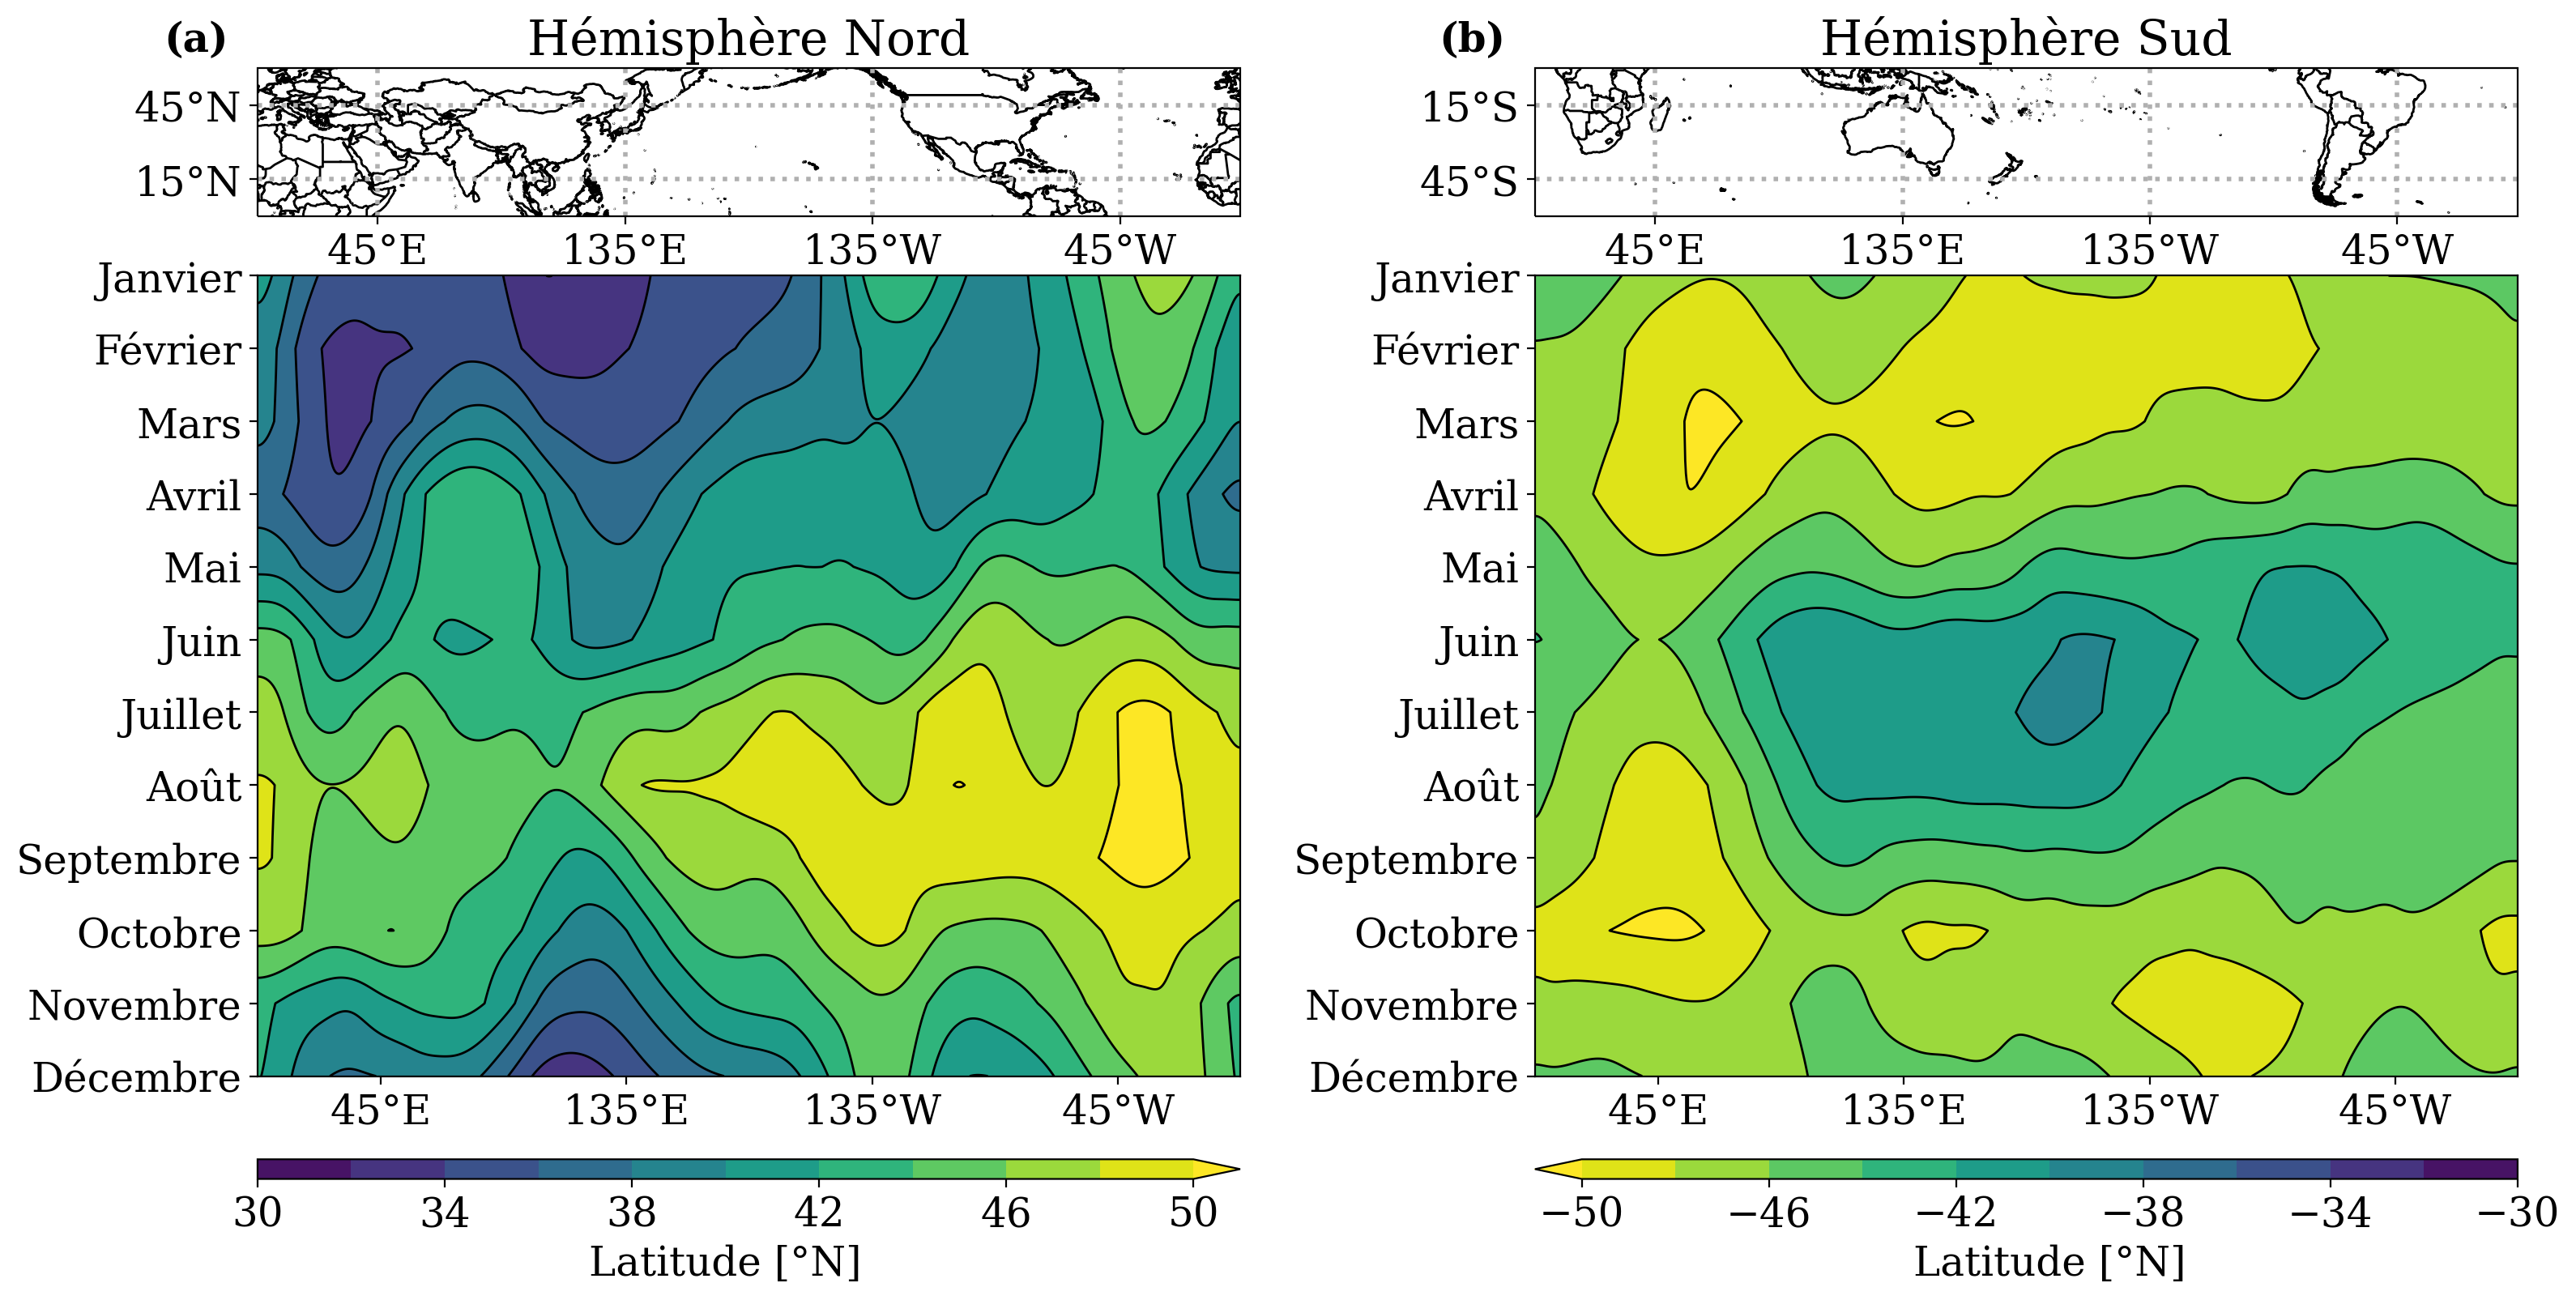
\includegraphics[width=\textwidth]{geopdy_clim_NH_SH.png}
    \caption{Diagramme de Hovmöller de la climatologie mensuelle de la latitude du gradient maximal de géopotentiel à \hPa{200}, lissée par un filtre gaussien,
    pour l'hémisphère nord (a) et sud (b), calculée de \num{1980} à \num{2020} avec la réanalyse ERA5. Contours de \ang{30}N à \ang{50}N (respectivement Sud)
    par pas de \ang{2}. L'utilisation de contours dans cette figure rend le diagramme imparfaitement périodique.}
    \label{fig:geopdy_clim}
\end{figure}

Avec ce filtre, le FAR intégré sur la période \num{1981}~--~\num{2019} et sur les cinq bassins d'activité vaut \prct{36}, soit seulement 12 points de
pourcentage de plus qu'avec le $V_U^T$. Ses performances à l'échelle des bassins d'activité sont toutefois très variables. Le filtre du gradient de géopotentiel
est particulièrement efficace dans le bassin WPac, où le taux de faux positivité est réduit à \prct{10} (respectivement \prct{14} dans
\cite{dulac_assessing_2023}). Dans le bassin EPac, il est à peu près aussi efficace que le $V_U^T$ avec \prct{21} (respectivement \prct{20}). Dans le NAtl et
SInd, le filtre du gradient de géopotentiel produit un FAR de respectivement \prct{37} et \prct{39} (contre respectivement \prct{20} et \prct{21} pour le
$V_U^T$), soit un taux de faux positif presque doublé. C'est toutefois dans le SPac que le filtre considéré dans cette section est le moins efficace, avec un
FAR de \prct{71}, c'est à dire du même ordre que le POD dans ce bassin. Ces performances variables, insuffisantes dans le cas du SPac, s'expliquent par le fait
que le champ de $\partial Z_{200} / \partial \phi$ n'est pas suffisamment lisse en latitude, si bien que la latitude du gradient oscille entre le jet polaire
---~situé aux alentours de \ang{60}~--- et le jet subtropical, autour de \ang{30}. Si c'est effet n'est pas visible sur sur les
\cref{fig:ophelia_z200,fig:geopdy_clim}, c'est parce que ces dernières ont fait l'objet d'un lissage agressif. Sur la \cref{fig:ophelia_z200}, le gradient est
calculé sur le champ de géopotentiel moyenné sur \num{7} jours. Sur la \cref{fig:geopdy_clim}, les moyennes climatologiques pour chaque mois de la latitude du
gradient maximum sont lissées par filtre gaussien. La \cref{fig:geopdy_random} illustre ce problème à travers six exemples tirés aléatoirement dans l'hémisphère
sud sur la saison cyclonique 2019. Précisons que les champs de $\partial Z_{200} / \partial \phi$ qui y sont présentés sont calculés sur la hauteur
géopotentielle elle-même lissée spatialement avec une fenêtre glissante carrée de côté 11, conformément à l'implémentation online qui en est faite dans le
schéma de détection. Cette figure montre que la chute de la hauteur géopotentielle avec la latitude n'est pas définie de façon suffisamment nette partout,
résultant en une latitude du gradient maximal en dents de scie. L'effet est amplifié pour les cas où deux bandes de fort gradient sont superposées. Sur la
\cref{fig:geopdy_random}, cela est particulièrement visible pour la date du 2018--08--26 (1\iere~ligne 2\ieme~colonne) et la date du 2019--06--29 (2\ieme~ligne
1\iere~colonne), et plus localement pour la date du 2019--06--24 (1\iere~ligne 1\iere~colonne) entre \ang{0}E et \ang{180}, ou encore au 2019--04--21
(1\iere~ligne 3\ieme~colonne) entre \ang{180} et \ang{120}W. Dans ces cas, la latitude du gradient maximum saute d'un courant atmosphérique à l'autre, séparés
de \ang{30} l'un de l'autre. Parmi les autres dates, il apparaît que le gradient à la limite des subtropiques n'est souvent pas suffisamment fort par rapport au
gradient dans les latitudes plus proches du pôle, si bien que la latitude du gradient maximal frôle localement la limite méridionale du domaine de
fonctionnement du schéma de détection, \ang{60}S, comme par exemple à la date du 2018--09--12 (2\ieme~ligne 2\ieme~colonne), autour de \ang{60}E (bassin SInd)
ainsi qu'entre \ang{120}W et \ang{60}W (SPac), ce qui est essentiellement équivalent à ne pas avoir de filtre.
%
\begin{figure}[tb]
    \centering
    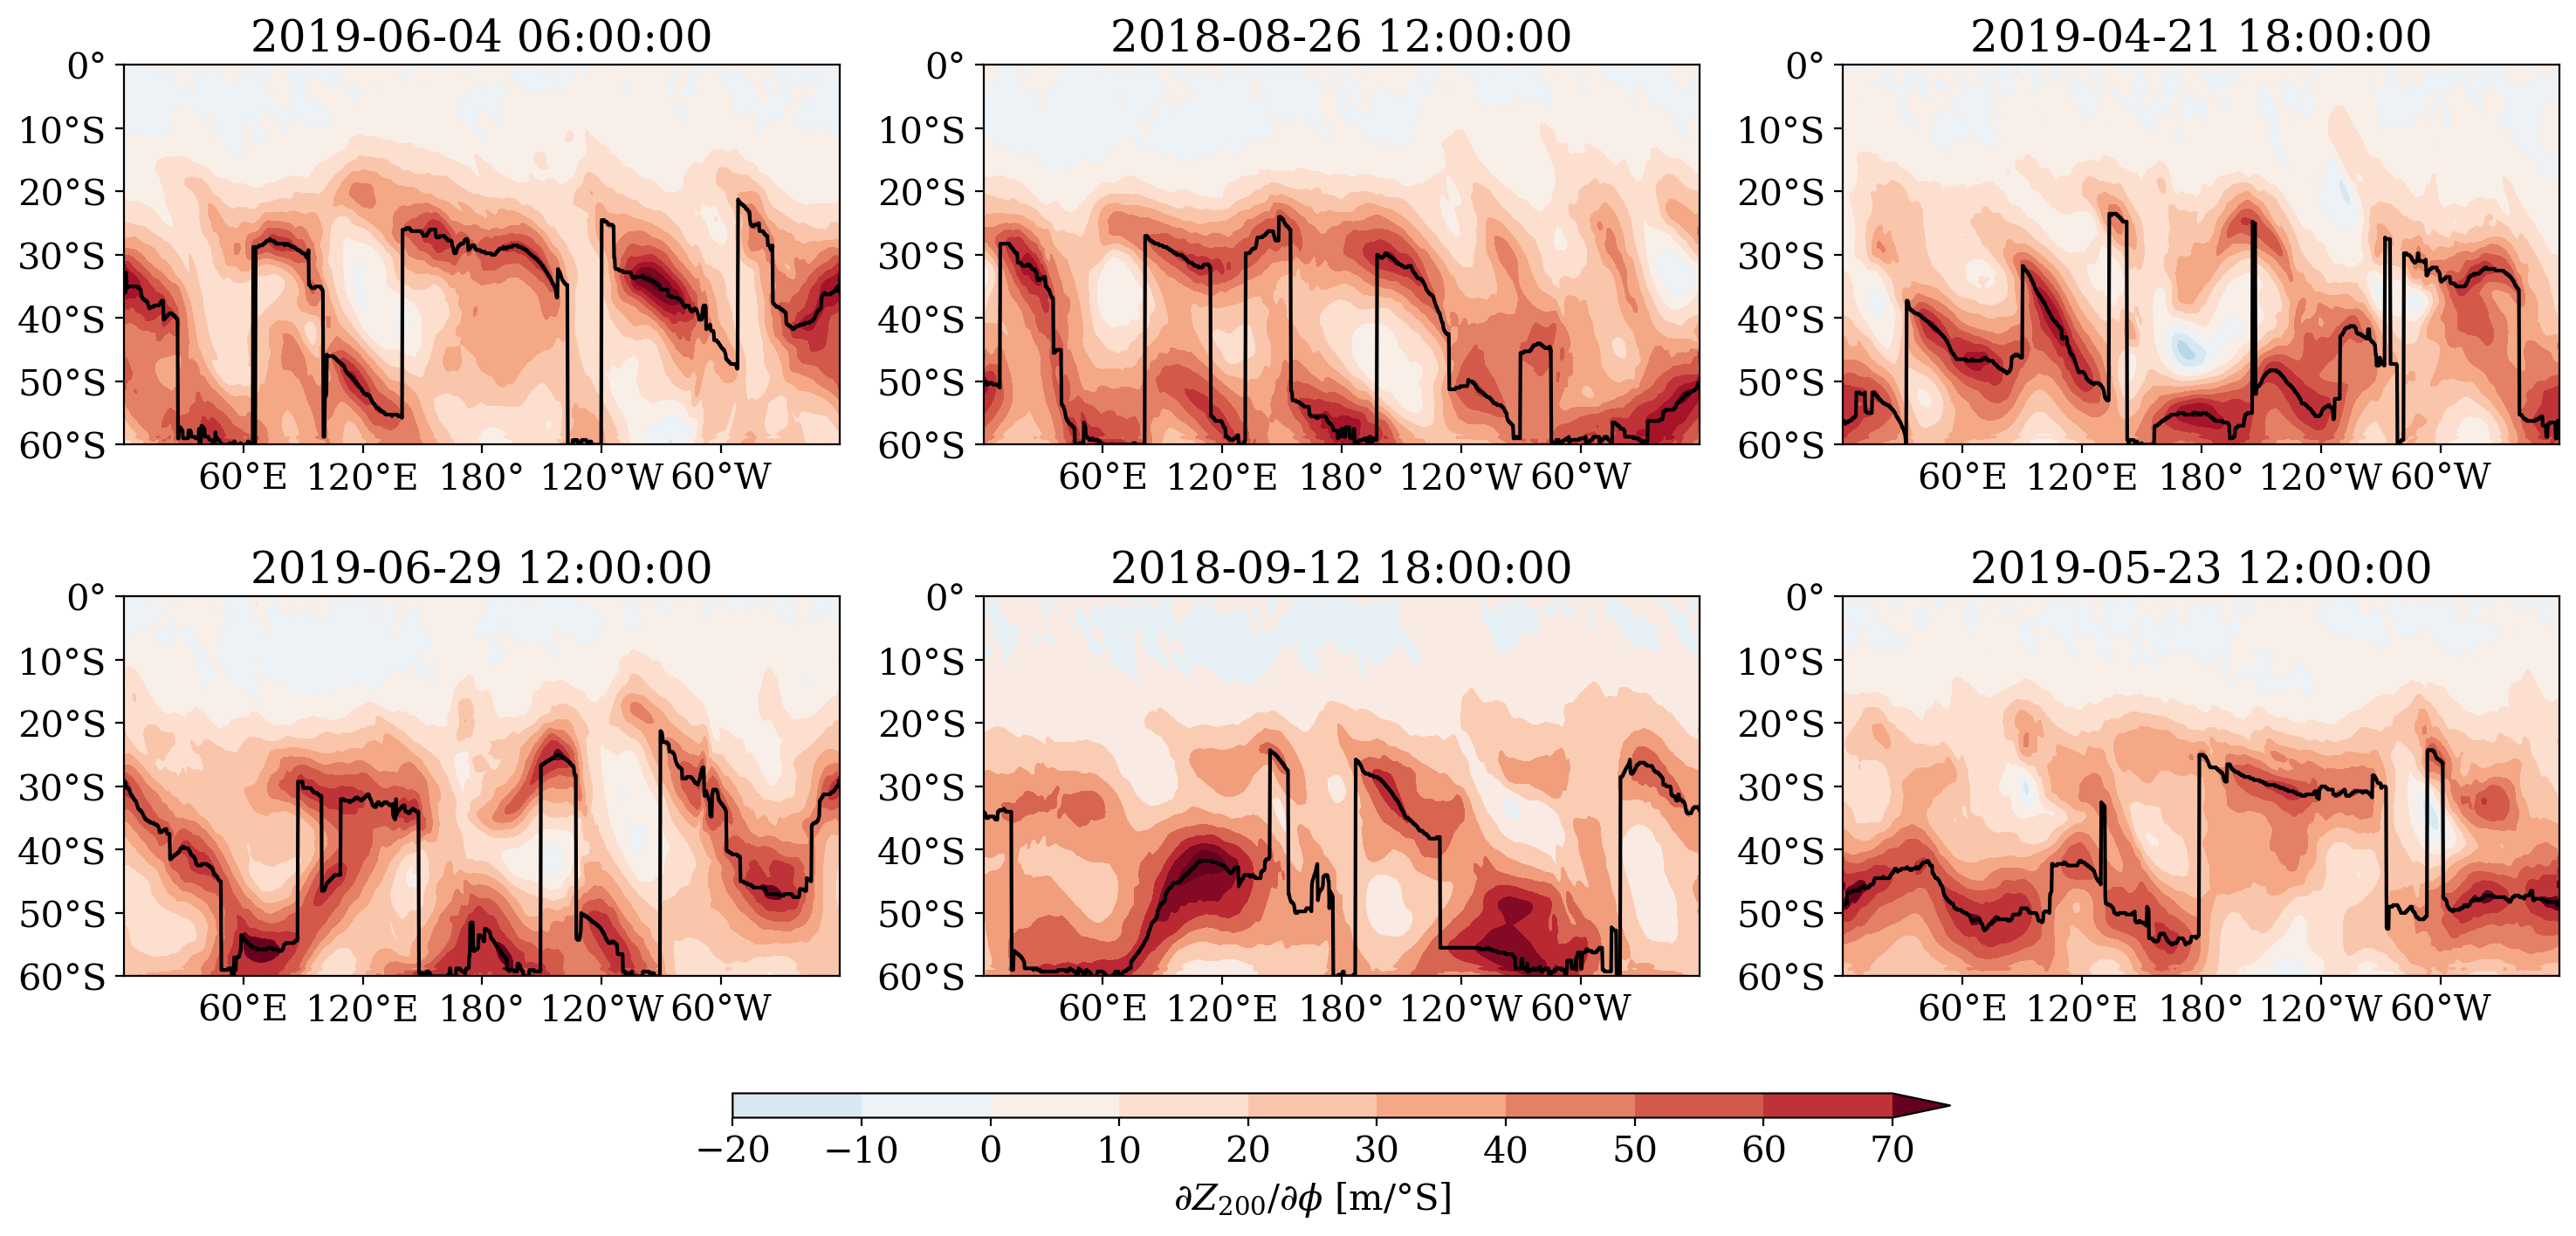
\includegraphics[width=\textwidth]{geopdy_random_dates.png}
    \caption{Gradient méridional de la hauteur géopotentielle à \hPa{200} pour 6 échéances tirées aléatoirement dans la saison cyclonique 2019 de l'hémisphère
    sud dans la réanalyse ERA5. Le tracé noir relie les points de gradient maximal pour chaque longitude.}
    \label{fig:geopdy_random}
\end{figure}

\subsubsection*{Filtre du jet subtropical}

Le filtre du gradient de géopotentiel à \hPa{200} vise essentiellement à définir un courant jet comme limite méridional des tropiques. D'autres travaux ont
employé une approche similaire basée sur un diagnostique différent du jet subtropical, en lieu et place d'un seuil fixe en latitude
\parencite{tory_projected_2013,tory_sea_2015,bell_statistical_2018}, dont la formulation est reprise dans \cite{bourdin_intercomparison_2022}. Spécifiquement,
le diagnostique du jet subtropical, ou STJ (\textit{Subtropical Jet}) consiste à lisser les composantes horizontales $u$ et $v$ du vent à \hPa{200} avec une
fenêtre glissante de 30 jours, puis à déterminer la région dans laquelle le module du vent est supérieur à \ms{25} et où la composante zonale $u$ est supérieure
à \ms{15}. Le seuil en latitude du filtre est ensuite défini en prenant la limite équatoriale de la zone où ces conditions sont réunies, où en interpolant
linéairement entre les deux points les plus proches dans l'éventualité où le STJ ne serait pas défini sur une tranche de longitude donnée, et en interpolant
temporellement en dernier recours si aucun point ne remplit les critères à un pas de temps donné. 

La \cref{fig:STJ_random} illustre le fonctionnement du filtre du STJ, en montrant pour les trois dates prises comme exemple sur la 1\iere~ligne de la
\cref{fig:geopdy_random}, la région où $\sqrt{u^2 + v^2} > \ms{25}$ et $u > \ms{15}$, accompagnée de la limite équatoriale de cette zone indiquée par les tirets
rouges. Le diagnostique du jet subtropical apparaît comme nettement plus lisse que le filtre du gradient de géopotentiel, et est également situé plus proche de
l'équateur, même en mettant de côté l'effet dents de scie du gradient de $Z_{200}$. La proximité avec l'équateur s'explique par la caractéristique du STJ à
prendre la limite équatoriale plutôt que le maximum du champ, tandis que le lissage sur 30 jours glissants permet d'atteindre une meilleure homogénéité en
longitude. En effet la 2\ieme~ligne de la \cref{fig:STJ_random} présente le diagnostique établi sur les trois mêmes dates sur les composantes du vent non
lissées et montre une plus grande irrégularité dans le placement du STJ. Sur la 3\ieme~colonne, à la date du 2019--04--21, cela se traduit par le même effet que
pour le filtre précédent, avec des chutes brutales de la limite équatoriale du jet vers le pôle. Le diagnostique réalisé sans lissage temporel met illustre la
grande proximité conceptuelle entre les deux filtres, puisque la structure des régions remplissant les deux conditions correspond très fidèlement aux zones de
fort gradient de géopotentiel présentées sur la 1\iere~ligne de la \cref{fig:geopdy_random}, l'intensité des courants jets à \hPa{200} étant directement
proportionnelle à $\partial Z_{200} / \partial \phi$. Il en résulte que le lissage temporel préalable des champs concernés constitue la différence fondamentale
entre les deux méthodologies.

\begin{figure}[tb]
    \centering
    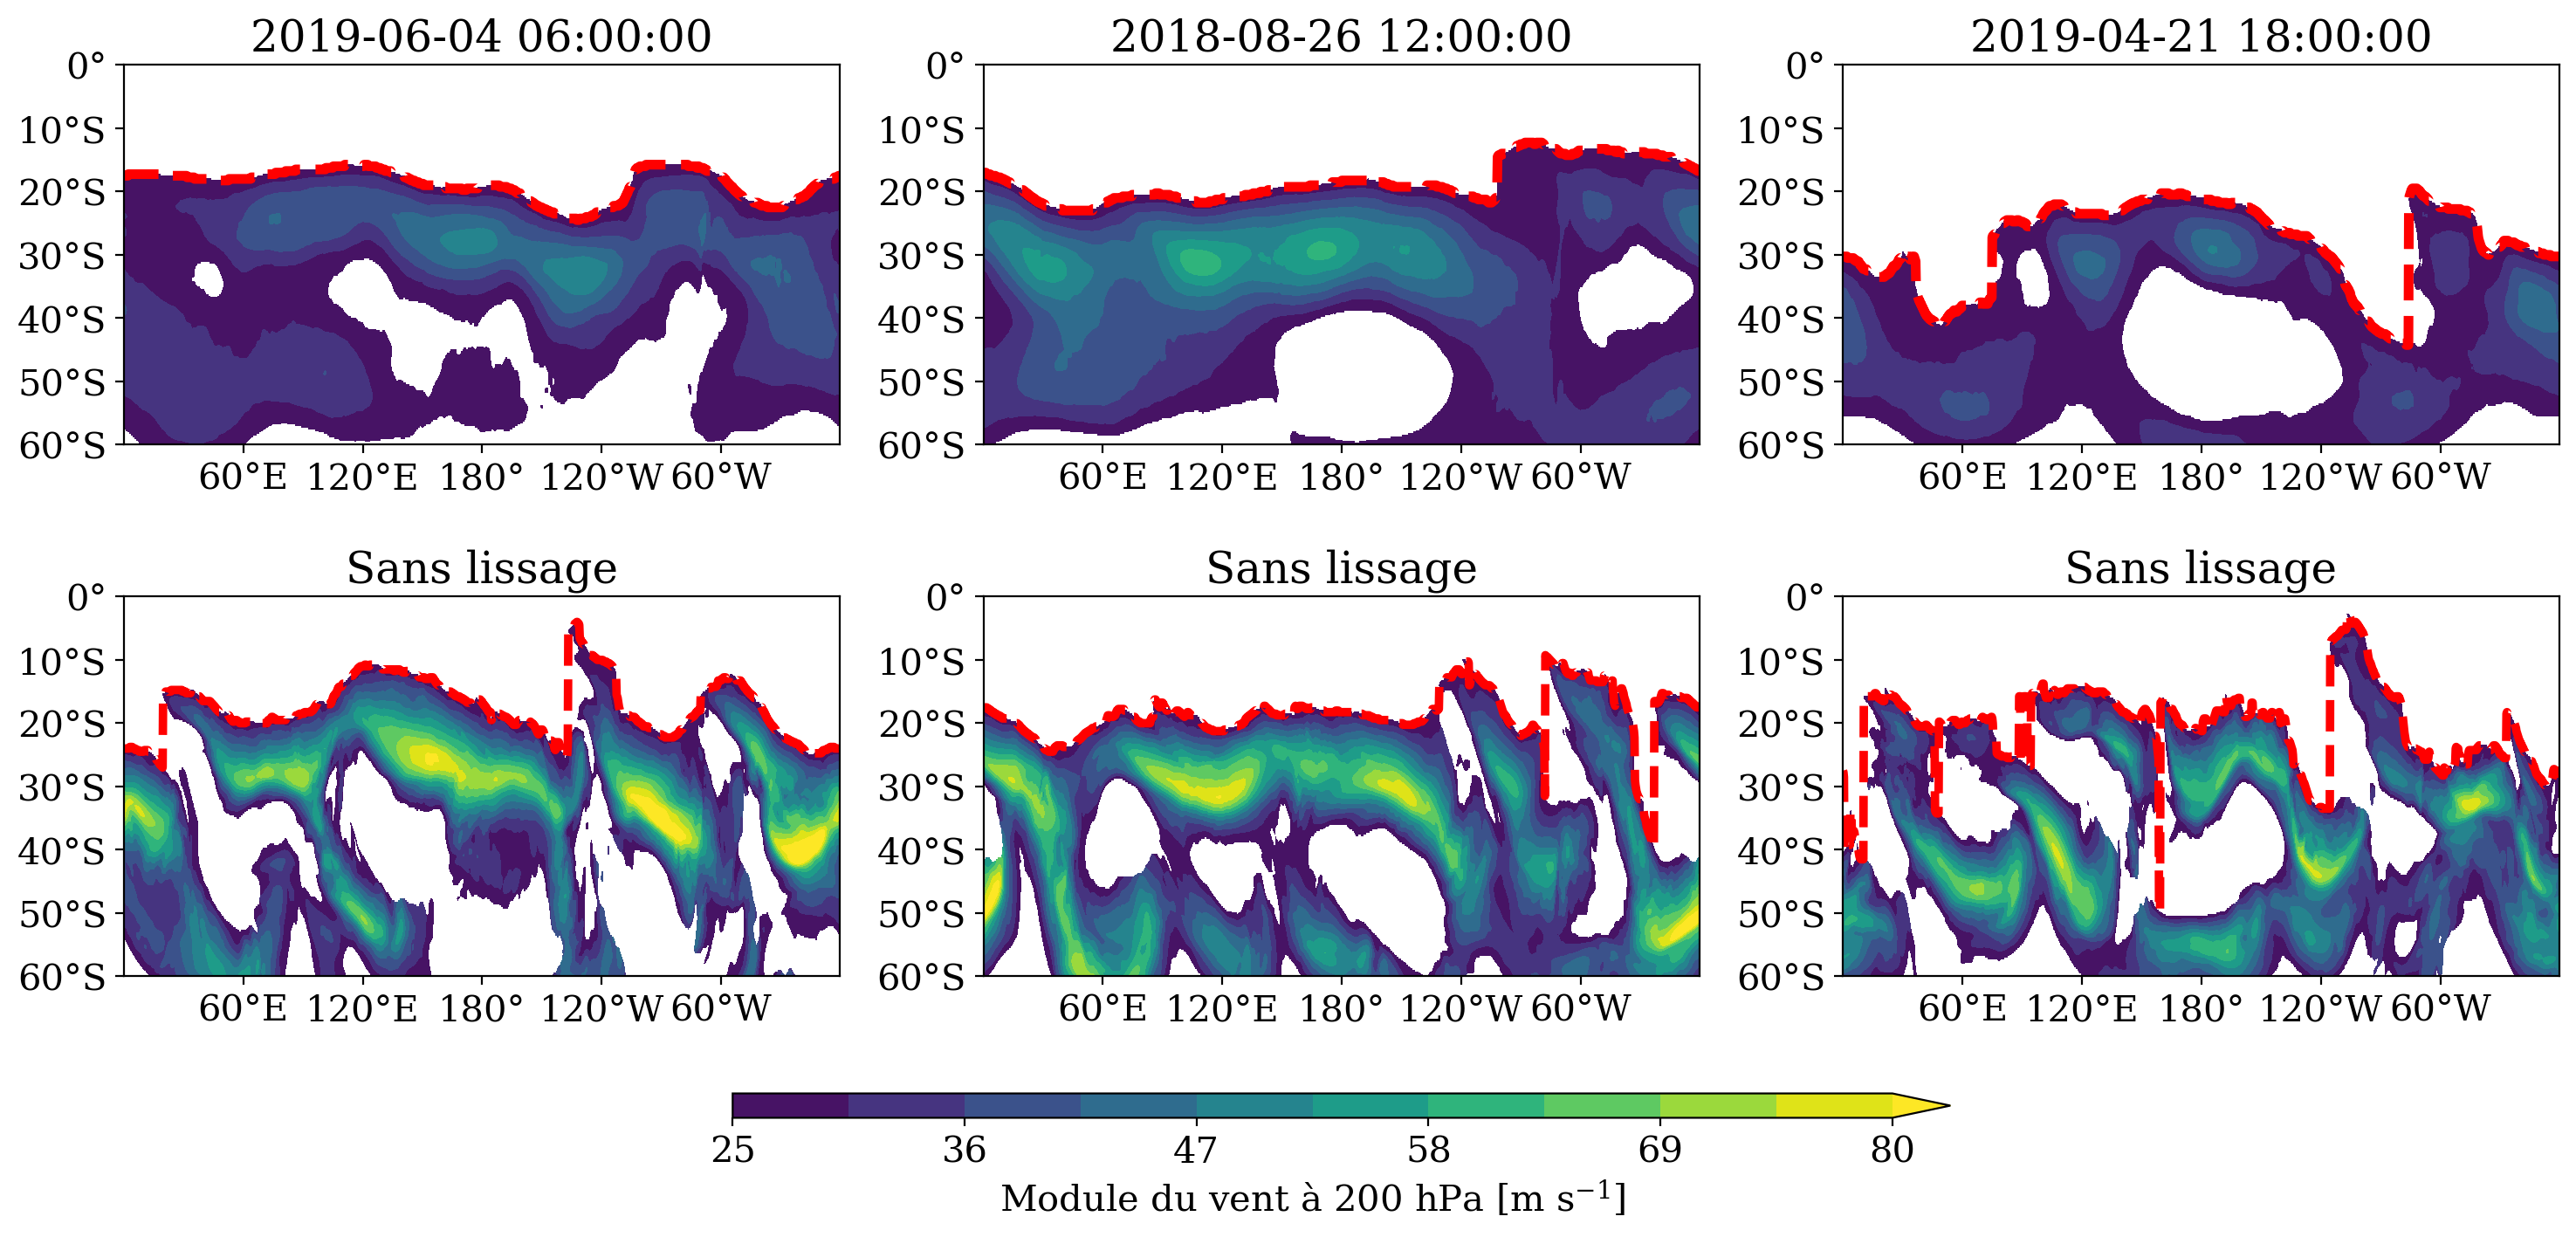
\includegraphics[width=\textwidth]{STJ_mask_random.png}
    \caption{Principe de fonctionnement du diagnostique du jet subtropical pour les trois dates de la première ligne de la \cref{fig:geopdy_random}. La seconde
    ligne applique le diagnostique aux trois mêmes dates avec le vent instantané non lissé. Le tracé en tirets rouge indique la limite équatoriale du jet
    subtropical ainsi déterminé.}
    \label{fig:STJ_random}
\end{figure}

Les performances du STJ sont discutées dans \cite{bourdin_intercomparison_2022}, et l'efficacité de ce système n'est pas à démontrer. En particulier,
\cite{bourdin_intercomparison_2022} mesure un taux de faux positifs à \prct{15} avec le STJ sur le traqueur du CNRM à l'échelle globale. Notons que le STJ
appliqué au traqueur CNRM dans \cite{bourdin_intercomparison_2022} produit par ailleurs un FAR d'environ \prct{30} dans le bassin SPac, ce qui est en dessous
des \prct{42} notés dans \cite{dulac_assessing_2023} avec le $V_U^T$. \cite{bourdin_intercomparison_2022} justifient également le choix du STJ par rapport au
$V_U^T$ par le coût supplémentaire en probabilité de détection que ce dernier représente. Chercher à diagnostiquer objectivement la présence d'un courant jet
peut néanmoins parfois mener à des résultats inattendus qui peuvent alors compromettre la définition du seuil en latitude pour le schéma de détection de TC. La
\cref{fig:geopdy_and_STJ} présente trois cas sélectionnés durant l'année 2017 dans l'hémisphère nord qui illustrent cela, avec d'un côté de la figure une carte
de l'hémisphère montrant le seuil méridional déterminé par les deux méthodologies, et l'autre côté montrant le courant diagnostiqué à cette échéance. Le premier
cas (1\iere~ligne) montre un STJ diagnostiqué (encadré de droite) épars avec des parcelles de vent fort à différentes latitudes, si bien que la limite
équatoriale subit des sauts soudains de plus de \ang{20}. Dans cet exemple, trois sauts successifs sont constatés dans le bassin EPac autour de \ang{150}W,
suivi d'une rupture additionnelle dans le bassin NAtl, à \ang{30}W. Ces ruptures sont comparables dans leur amplitude aux sauts constatés dans le filtre du
gradient de géopotentiel. Le second cas (2\ieme~ligne) présente un jet subtropical presque absent, avec deux parcelles principales dont le vent ne dépasse pas
\ms{40}, l'un autour de \ang{60}E et l'autre centré sur \ang{60}W. Les cas où le courant jet est faible et donc imparfaitement défini sont nombreux durant la
saison estivale, le gradient de température Nord-Sud étant affaibli par les fortes températures dans les latitudes subtropicales en été. Dans ces cas là, le
seuil en latitude issu du diagnostique du STJ est soit parasité par des parcelles de vent éparses, comme dans le premier cas, où bien particulièrement lisse car
interpolé sur une grande partie du domaine, comme dans le second. Le troisième cas (3\ieme~ligne), quant à lui, présente une situation où du vent fort est
identifié au niveau de l'équateur, causant une chute de la latitude issue du diagnostique à \ang{0}N. Ces cas semblent plus rare, et apparaissent limités à la
saison hivernale, lorsque le STJ est au plus fort, et l'activité cyclonique est nulle. Bien que ce cas concerne ici l'hémisphère nord, l'hémisphère sud est lui
aussi concerné par ces situations qui témoignent de la difficulté à diagnostiquer objectivement le courant jet ---~toute méthode de détection objective étant
nécessairement sujette à des erreurs.

\begin{figure}[tb]
    \centering
    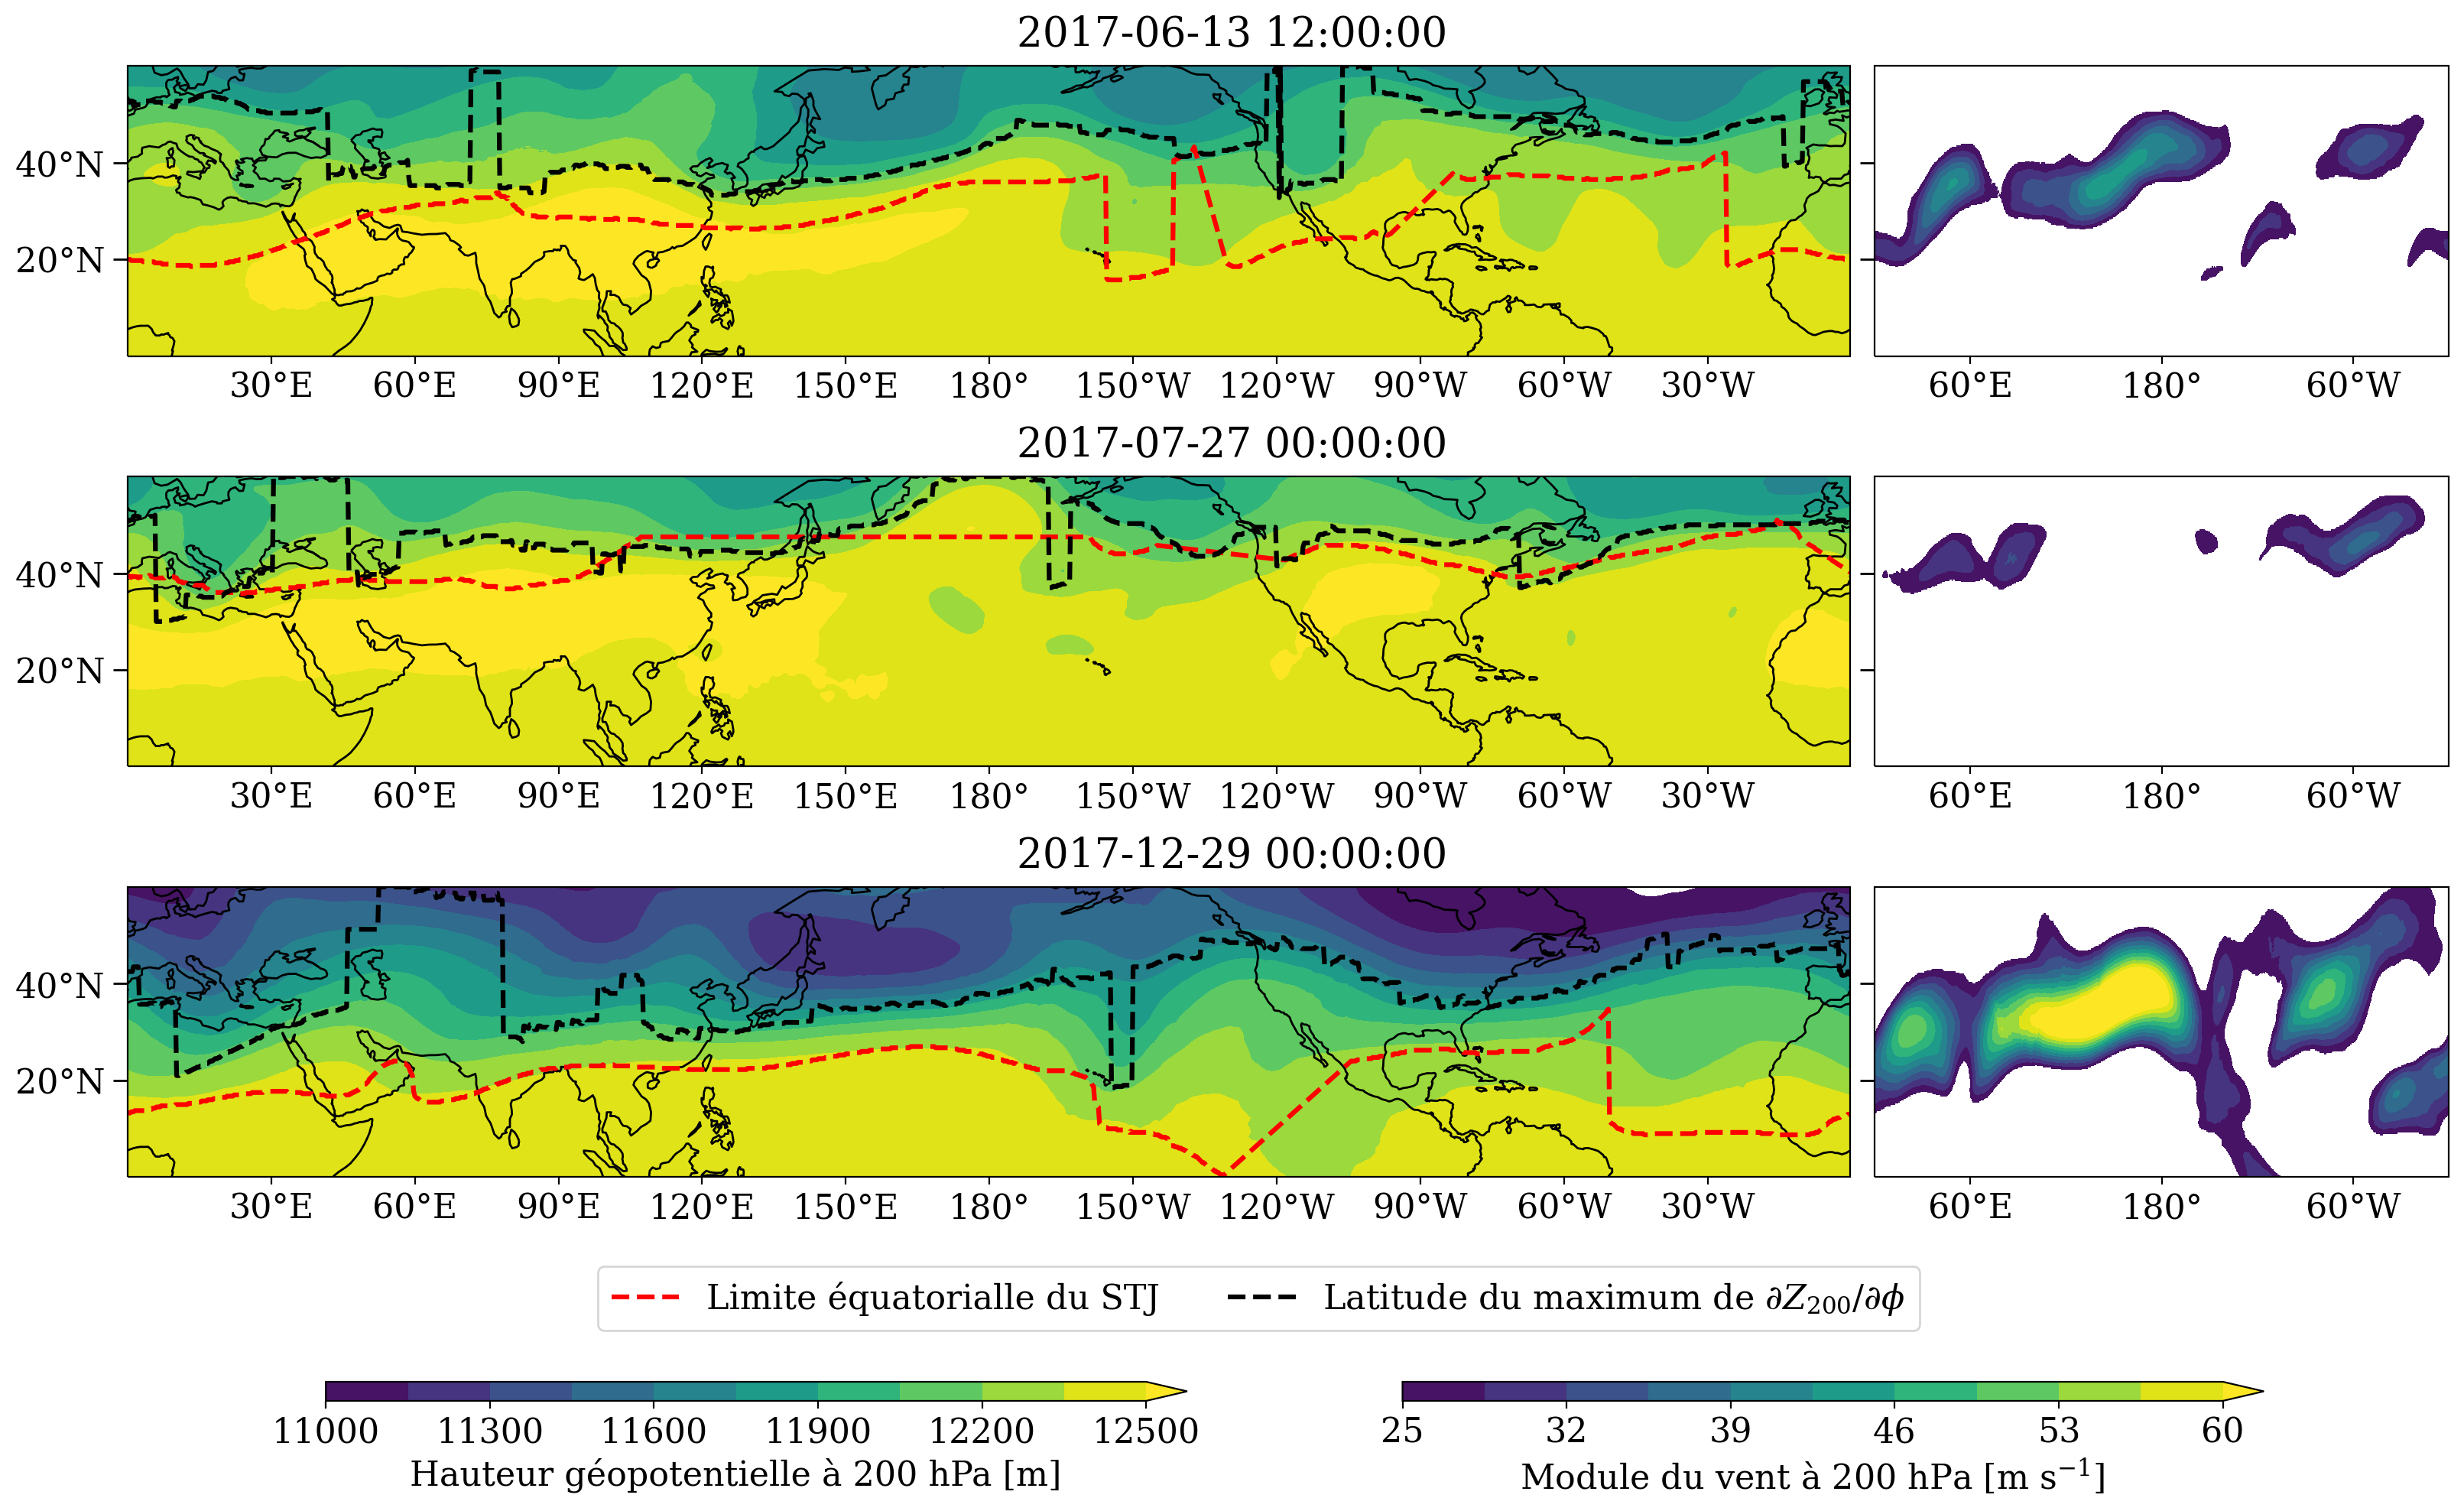
\includegraphics[width=\textwidth]{geopdy_and_STJ.png}
    \caption{Comparaison de la latitude du jet subtropical avec la latitude du maximum de gradient de géopotentiel pour trois échéances de la saison cyclonique
    2017 de l'hémisphère nord dans lesquels le STJ n'est pas clairement défini. La carte de gauche présente les deux limites en latitude sur fond du champ de
    hauteur géopotentielle à \hPa{200}, tandis que l'encadré de droite présente le jet subtropical diagnostiqué, dont la limite équatoriale détermine le tracé rouge
    sur la carte. Pour chaque date, les deux encadrés couvrent l'entièreté de l'hémisphère nord jusqu'à \ang{60}N, en dépit de leur largeur différentes.}
    \label{fig:geopdy_and_STJ}
\end{figure}

\subsubsection*{Conclusion}

Le filtre du gradient méridional de hauteur géopotentielle à \hPa{200} appliqué au schéma de détection de cyclones tropicaux du CNRM fournit des résultats
variables selon les bassins, avec de bonnes performances dans les bassin WPac et EPac, mais des résultats mitigés dans le NAtl et le SInd. Il est cependant
extrêmement inefficace dans le bassin SPac. Outre ces résultats, il apparaît que les champs de $\partial Z_{200} / \partial \phi$ ne sont pas suffisamment
lisses pour permettre leur utilisation dans l'objectif de filtrer les tempêtes extratropicales, puisque la latitude du gradient maximale est sujette à des
ruptures fréquentes conduisant à une limite méridionale en dents de scie.

Le filtre du STJ quant à lui conduit à de biens meilleures performances, le seuil en latitude qui en résulte étant souvent bien plus proche de l'équateur, et
accomplit cela principalement grâce au lissage temporel des composantes du vent à \hPa{200}. Le lissage sur 30 jours glissants est nécessaire pour espérer
mesurer un courant jet bien défini, mais tout type de lissage temporel rend une implémentation online impossible, le schéma de détection n'ayant connaissance
que de l'état instantané de l'atmosphère. Ce filtre ne peut donc s'appliquer que sous la forme d'un post-traitement. Par ailleurs, diagnostiquer de manière
objective la présence du courant jet n'est pas toujours facile, notamment car celui-ci est à son plus faible durant la saison chaude, qui correspond pourtant à
la plus forte activité cyclonique, et donc à la saison où le filtre est le plus nécessaire. Si l'interpolation spatiale et temporelle de la limite
équatoriale du STJ permet de garantir le bon fonctionnement du filtre dans ces cas là, la solution n'est toutefois pas pleinement satisfaisante.

Pour ces raisons, et en dépit du coût supplémentaire en probabilité de détection, le filtre basé sur le paramètre $V_U^T$ de \cite{hart_cyclone_2003} a été
préféré pour le schéma de détection du CNRM dans \cite{dulac_assessing_2023}. Outre le fait qu'il ne dépend que des champs instantanés de l'atmosphère, il
présente aussi l'avantage d'être défini en toute circonstance et de s'appliquer à tous les systèmes détectés. Cela signifie qu'il peut filtrer des systèmes peu
intenses dans les tropiques également. C'est notamment pour cette raison que \cite{bourdin_intercomparison_2022} indiquent que le filtre $V_U^T$ est plus
efficace que le STJ lorsqu'appliqué au traqueur OWZ \parencite{tory_importance_2013}, les systèmes de moyennes latitudes n'étant pas majoritaires dans la
population de faux positifs de ce schéma de détection sur ERA5. Si la définition du filtre du $V_U^T$ rend possible une implémentation online, ce dernier a été
appliqué comme post-traitement dans \cite{dulac_assessing_2023} pour des raisons de facilité. Une implémentation online dans le schéma de détection du CNRM est
envisagée, mais nécessite un travail de refonte approfondi du traqueur. En particulier, il semble nécessaire de comprendre précisément pourquoi les critères de
détection \textbf{PW} et \textbf{PT}, détaillés dans la \cref{sec:papier_data_methods} et qui diagnostiquent la présence d'un profil vertical de température et
de vent, échouent à filtrer les systèmes extratropicaux là où le paramètre $V_U^T$ y parvient, la combinaison des deux paramètres diagnostiquant
fondamentalement la même chose que le test de \citeauthor{hart_cyclone_2003}.

\subsection{Métriques d'évaluation de la similarité des trajectoires}\label{sec:similarité}

\subsubsection*{Introduction}

Les travaux réalisés dans \cite{dulac_assessing_2023} et présentés dans la \cref{sec:papier} font appel aux notions de FAR et POD pour évaluer la performance de
le schéma de détection de TC du CNRM. Le calcul du POD s'appuie sur un algorithme qui associe les trajectoires détectées dans ERA5 à celles présentes dans la
base de données IBTrACS par correspondance spatio-temporelle. Si en moyenne le taux de recouvrement des trajectoires appariés (\textquote{\textit{matched}} dans
\cite{dulac_assessing_2023}) ---~c'est à dire le nombre de points ERA5 situés à moins de \km{300} d'IBTrACS rapporté au nombre d'échéances de la trajectoire
IBTrACS, tel que défini dans la \cref{sec:papier_data_methods}~--- est de \prct{68} (médiane à \prct{71}), il suffit dans l'absolu d'un seul pas de temps
remplissant la condition pour que la trajectoire ERA5 soit appariée à une trajectoire présente dans les observations, et donc pour que la trajectoire détectée
contribue au POD. Ce cas est néanmoins rare puisqu'il concerne en tout et pour tout \num{7} paires de trajectoires ERA5 / IBTrACS, mais on note cependant que
près de \prct{4} de nos trajectoires ERA5 ont un taux de recouvrement inférieur ou égal à \prct{25}. Par ailleurs, le taux de recouvrement des couples de
trajectoires ainsi formés tend à augmenter avec l'intensité des cyclones observés, comme le montre la \cref{fig:coverage_ratio} encadré (a), et qui s'explique
par le fait que les cyclones les plus intenses sont les plus facilement détectables par le traqueur. Cette tendance à de meilleurs recouvrements pour les
cyclones les plus forts n'empêchent pas une certaine dispersion des valeurs. Par exemple \prct{5} des trajectoires appariés à des TC de catégorie \num{3} ont un
taux de recouvrement inférieur ou égal à \prct{31}. Une partie de la variance dans ces scores peut s'expliquer par le fait que le traqueur du CNRM est
susceptible de manquer le début et la fin du cycle de vie des trajectoires observées, en dépit du mécanisme de relaxation des paramètres utilisé dans le schéma
de détection \parencite[][Figure 8]{bourdin_intercomparison_2022}, auquel cas le recouvrement s'en voit mécaniquement réduit. L'autre facteur est que les
trajectoires ERA5 peuvent localement s'éloigner à plus de \km{300} d'IBTrACS. La \cref{fig:coverage_ratio} encadré (b) montre la distribution de la fraction des
points ERA5 situés à plus de \km{300} des observations pour chaque paire de trajectoire et montre qu'en moyenne \prct{5.8} des points détectés par le traqueur
parmi les trajectoires appariés à IBTrACS sont au delà de la limite d'appariement. De plus, \prct{5} des trajectoires détectées dans ERA5 ont une fraction
divergente d'au moins \prct{26}. Par conséquent, la trajectoire détectée dans la réanalyse n'est pas toujours identique à celle du catalogue des best tracks,
soit parce que le traqueur n'en détecte qu'une partie, soit parce que la trajectoire détectée diverge des observations, ou encore par une combinaison quelconque
de ces deux éléments. Enfin, bien que le taux de recouvrement donne une indication sur la similarité des deux trajectoires, il n'apporte pas d'information sur
les variations locales dans la direction de déplacement, ni ne quantifie les cas où la trajectoire ERA5 dépasse celle observée en amont ou en aval, si bien que
ce dernier n'est pas adapté pour évaluer quantitativement la ressemblance entre les trajectoires détectées dans la réanalyse et celles issues des observations.

\begin{figure}[tb]
    \centering
    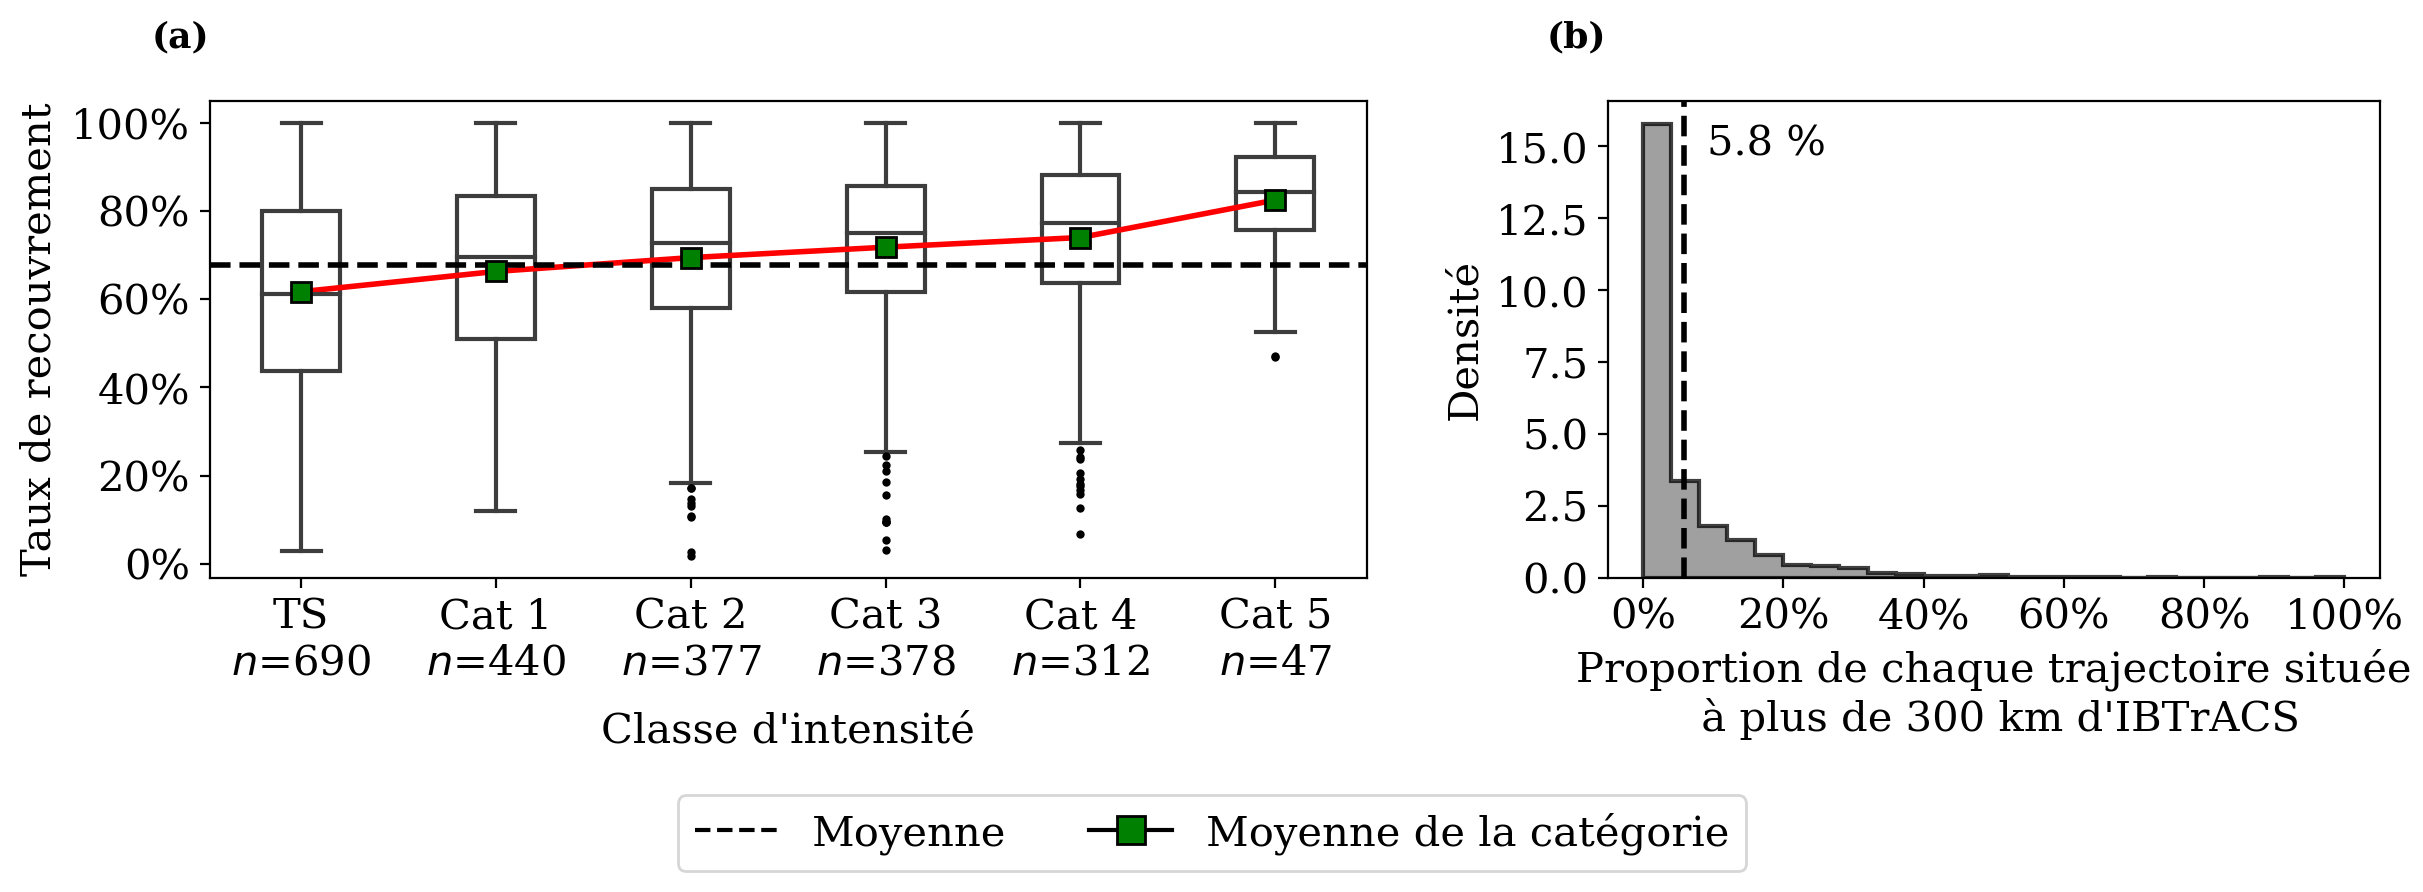
\includegraphics[width=\textwidth]{coverage_ratio_and_missed.png}
    \caption{\textbf{(a)} Distributions des taux de recouvrement des trajectoires appariées entre ERA5 / IBTrACS pour chaque classe d'intensité des TC observés.
    \textbf{(b)} Histogramme de la fraction de points détectés situés à plus de \km{300} d'IBTrACS parmi les trajectoires appariés.}
    \label{fig:coverage_ratio}
\end{figure}

Il existe dans la littérature des algorithmes d'évaluation de la similarité de séries temporelles
\parencite{faloutsos_fast_1994,das_finding_1997,frentzos_indexbased_2007}, mais ces derniers sont plutôt conçus pour des séries uni-dimensionnelles que pour des
trajectoires spatiales car sont souvent basés sur la distance euclidienne qui les sépare. \cite{nakamura_shapebased_2013} proposent une approche basée plutôt
sur la mesure de la similarité de la forme entre deux séries par l'analyse de l'angle formé par les séries, métrique nommée \textit{Angular Metric for Shape
Similarity} (AMSS). Bien que leur approche soit pleinement capable de s'appliquer à des trajectoires spatiales, certaines propriétés de leur métrique ne sont
pas pertinentes (voire pas souhaitables), dans le cas précis des trajectoires de cyclones tropicaux, telles qu'une forte résilience à un décalage temporel entre
les deux séries (pas applicable à des trajectoires appariées entre réanalyse et observations), ainsi qu'une robustesse à des changements isolés de direction.
Ces propriétés rendent par ailleurs leur algorithme très couteux en temps de calcul. Néanmoins, l'aspect novateur derrière les travaux de
\cite{nakamura_shapebased_2013} est repris ici, à savoir la décomposition de la trajectoire en série de vecteurs, détaillée ci-après. Dans cette section, trois
métriques de similarité des trajectoires sont définies et comparées sur le jeu de données issu de \cite{dulac_assessing_2023} et composé des trajectoires
détectées dans la réanalyse ERA5 qui sont appariées à des trajectoires historiques IBTrACS. En particulier, cette analyse vise à déterminer si le réglage des
seuils de détection du traqueur de TC du CNRM dans le but de maximiser le POD ne risque pas de produire des trajectoires peu ressemblantes, du fait de la
formulation de la condition nécessaire et suffisante à l'appariement de deux trajectoires.

\subsubsection*{La similarité angulaire}

\begin{figure}[htbp]
    \centering
    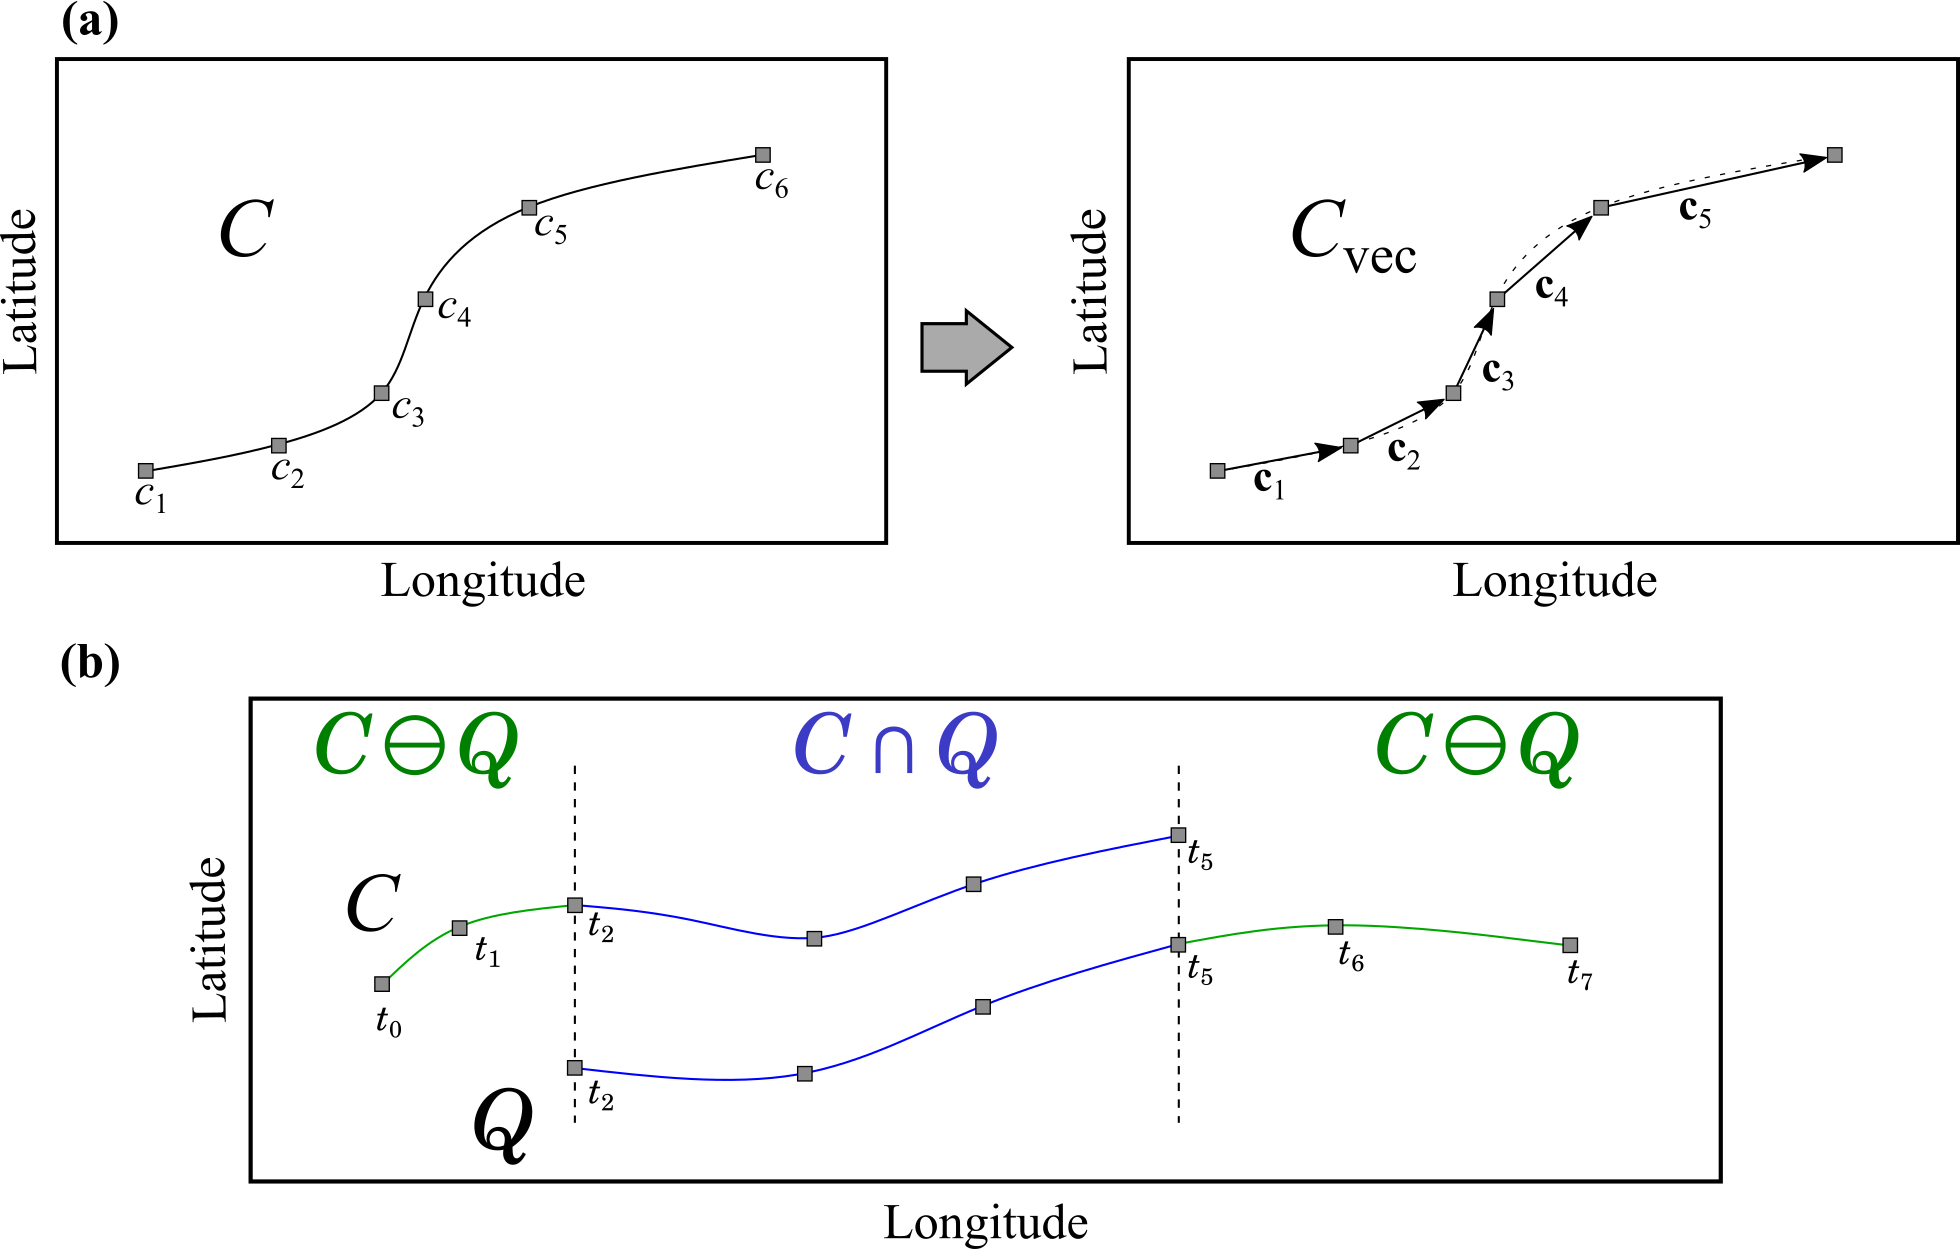
\includegraphics[width=\textwidth]{schema_vec_sequence.png}
    \caption{Représentation schématique de la décomposition d'une trajectoire $C$ en séquence de vecteurs de déplacements relatifs $C_{\text{vec}}$ (a),
    inspirée de \cite{nakamura_shapebased_2013}. Représentation visuelle de $C \cap Q$ et de $C \ominus Q$ (b). Dans cet exemple, $N_\cap = N_\ominus = 4$.}
    \label{fig:schema_trajectoires}
\end{figure}

Une trajectoire de cyclone tropical est une série temporelle composée des positions successives du système et accompagnées de diverses informations permettant
la caractérisation du système, telles que le vent maximum ou la pression centrale. Pour pouvoir évaluer la similarité entre deux trajectoires, on considère non
pas les positions discrètes du système, mais plutôt la série de vecteurs décrivant le déplacement relatif entre chaque position successive.

Reprenant le formalise de \cite{nakamura_shapebased_2013} ; soit $C$ une trajectoire de TC composée de $M+1$ pas de temps et définie par ses positions
$p_{1...M+1}$ sur une grille géo-référencée et aux temps $t_{1...M+1}$ :
%
\begin{align*}
    C &= ((p_1, t_1), (p_2, t_2), \ldots, (p_{M+1}, t_{M+1}))\\
      &= (c_1, c_2, \ldots, c_{M+1})
\end{align*}
%
Alors la série des vecteurs de déplacement équivalente $C_{\text{vec}}$ est donnée par :
\begin{align*}
    C_{\text{vec}} &= ((c_2 - c_1), (c_3 - c_2), \ldots, (c_{M+1} - c_M))\\
            &= (\mathbf{c}_1, \mathbf{c}_2, \ldots, \mathbf{c}_M)
\end{align*}
%
tel qu'illustré par la \cref{fig:schema_trajectoires}, encadré (a). Soit $Q_{\text{vec}}$ la série des vecteurs de déplacements d'une seconde trajectoire composée de
$M^\prime$ vecteurs. L'angle $\theta$ entre deux vecteurs individuels $\mathbf{c}_i$ et $\mathbf{q}_j$ issus respectivement de $C_{\text{vec}}$ et
$Q_{\text{vec}}$, et où $i$ et $j$ correspondent au même temps $t$ est donné par le produit scalaire des deux vecteurs. $\cos \theta$ est aussi appelé
similarité cosinus et est noté $S_C$ :
%
\begin{equation*}
    S_C(\mathbf{c}_i, \mathbf{q}_j) = \cos \theta = \frac{\mathbf{c}_i \cdot \mathbf{q}_j}{\lVert \mathbf{c}_i \rVert \lVert \mathbf{q}_j \rVert} \in [-1; 1] 
\end{equation*}
%
Ainsi la similarité cosinus caractérise l'angle formé par les vecteurs de déplacement issus de deux trajectoires à un instant donné. On peut ensuite définir la
distance angulaire, ou angle normalisé, qui est une distance formelle au sens où l'inégalité de Cauchy-Schwartz est respectée, par :
%
\begin{equation*}
    D_\theta = \frac{\theta}{\pi}
\end{equation*}
%
Et son complément, appelé similarité angulaire par :
%
\begin{equation*}
    S_\theta = 1 - D_\theta = 1 - \frac{\theta}{\pi} \in [0; 1]
\end{equation*}
%
C'est cette dernière distance $S_\theta$ qui est utilisée dans cette analyse. De cette façon, la plus faible similarité entre deux vecteurs est atteinte
lorsqu'ils sont parallèles mais de sens opposés, tandis que la similarité est maximale si deux vecteurs parallèles sont de même sens.

\subsubsection*{Métriques de similarité intégrée}\label{sec:definition_MAS}

Avant de définir les trois métriques, il est important de distinguer trois membres dans un couple de trajectoires appariées. En effet, la similarité angulaire
$S_\theta$ est définie ci-dessus pour deux vecteurs correspondants aux déplacements entre deux positions successives, pour deux trajectoires prises au même
temps $t$. Or, il est admis qu'un des deux vecteurs peut ne pas exister à cet instant si le schéma de détection n'a pas capturé l'entièreté de la trajectoire ou
au contraire si la trajectoire détectée est plus longue que celle observée, aussi bien en amont qu'en aval. On appelle donc l'intersection des trajectoires $C
\cap Q$ le sous-ensemble des pas de temps dans lequel les deux trajectoires co-existent et où chaque paire de points correspond au même temps $t$.
Réciproquement, l'union $C \cup Q$ contient l'entièreté des échéances consistuant le couple de trajectoires. Enfin, la différence symétrique des deux
trajectoires $C \ominus Q$ contient les pas de temps pour lesquels une seule trajectoire existe à la fois. La \cref{fig:schema_trajectoires} encadré (b)
illustre schématiquement ces notions.

En première approche, on peut définir la similarité intégrée entre deux trajectoires $C$ et $Q$ comme la moyenne de la similarité angulaire $S_\theta$ sur $C
\cap Q$, notée $\bar{S_\theta}^\cap$ (\textit{Mean Angular Similarity}, MAS):
%
\begin{equation}
    \bar{S_\theta}^\cap = \frac{1}{N_\cap} \sum_{i=1}^{N_\cap} S_\theta (\mathbf{c}_i, \mathbf{q}_i) \tag*{MAS$^\cap$}
\end{equation}
%
Cette première métrique de similarité se concentre donc sur les échéances où les deux trajectoires coexistent, les échéances non-détectées ainsi que celles en
trop par rapport aux observations n'étant pas compatiblisées.

Comme variante, on définit aussi le MAS sur l'union des deux trajectoires en remplaçant le dénominateur par $N_\cup = N_\cap + N_\ominus$. Cela revient
à considérer que les echéances sur $C \ominus Q$ ont une similarité angulaire artificiellement fixée à \num{0} :
%
\begin{equation}
    \bar{S_\theta}^\cup = \frac{1}{N_\cup} \sum_{i=1}^{N_\cap} S_\theta (\mathbf{c}_i, \mathbf{q}_i) \tag*{MAS$^\cup$}
\end{equation}
%
Ainsi, cette seconde métrique de similarité considère l'entièreté des deux trajectoires constituant le couple ERA5 / IBTrACS dans le calcul de la similarité, au
risque d'être très punitif si $N_\ominus \neq 0$.

On définit enfin une troisième métrique de similarité, pensée comme un hybride entre MAS$^\cap$ et MAS$^\cup$ dans sa prise en compte des échéances sur $C
\ominus Q$. Cette dernière métrique, nommée wMAS (\textit{weighted}), considère toujours comme nulle la similarité sur $C \ominus Q$, mais introduit deux
coefficients $w_1$ et $w_2$, en concurrence l'un contre l'autre, qui vont peser différemment sur $C \cap Q$ et $C \ominus Q$ respectivement, et qui s'expriment
comme fonction de $\bar{S_\theta}^\cap$ :
%
\begin{equation*}
\text{wMAS} = \frac{ w_1\sum_{i=1}^{N_\cap} S_{\theta}(\mathbf{c}_i, \mathbf{q}_i) }{ w_1 N_\cap + w_2 N_\ominus}\quad\quad \tag*{wMAS}
    \begin{cases}
        w_1 = a + \bar{S_\theta}^\cap \. , \;\; a \geq 0 \\
        w_2 = b - \bar{S_\theta}^\cap \. , \;\; b \geq 1 \\
    \end{cases}
\end{equation*}
%
Le wMAS vise à fournir une valeur quantitative du ressenti qualitatif de la similarité d'une paire de trajectoires, en ce sens que le plus la similarité moyenne
sur $C \cap Q$ est élevée, le moins la taille de $C \ominus Q$ a d'importance dans la similarité totale, et réciproquement. Le wMAS traduit donc l'idée
subjective que la similarité sur l'intersection des trajectoires peut compenser partiellement la différence de taille entre une trajectoire détectée associée à
une trajectoire observée. Le degré d'intensité de cette compensation (ou respectivement de pénalisation) peut être ajusté via les paramètres $a$ et $b$. Ici ces
paramètres sont empiriquement fixés à $a=1$ et $b=2$. Par construction, on a :
%
\begin{equation*}
    \text{MAS}^\cap \geq \text{wMAS} \geq \text{MAS}^\cup
\end{equation*}

\subsubsection*{Application}

La \cref{fig:MAS_Ndiff} présente la similarité des trajectoires appariées entre ERA5 et IBTrACS en fonction du nombre d'échéances non partagées entre elles,
c'est à dire pour les temps où une seule des deux est définie, $N_\ominus$.
%
\begin{figure}[htpb]
    \centering
    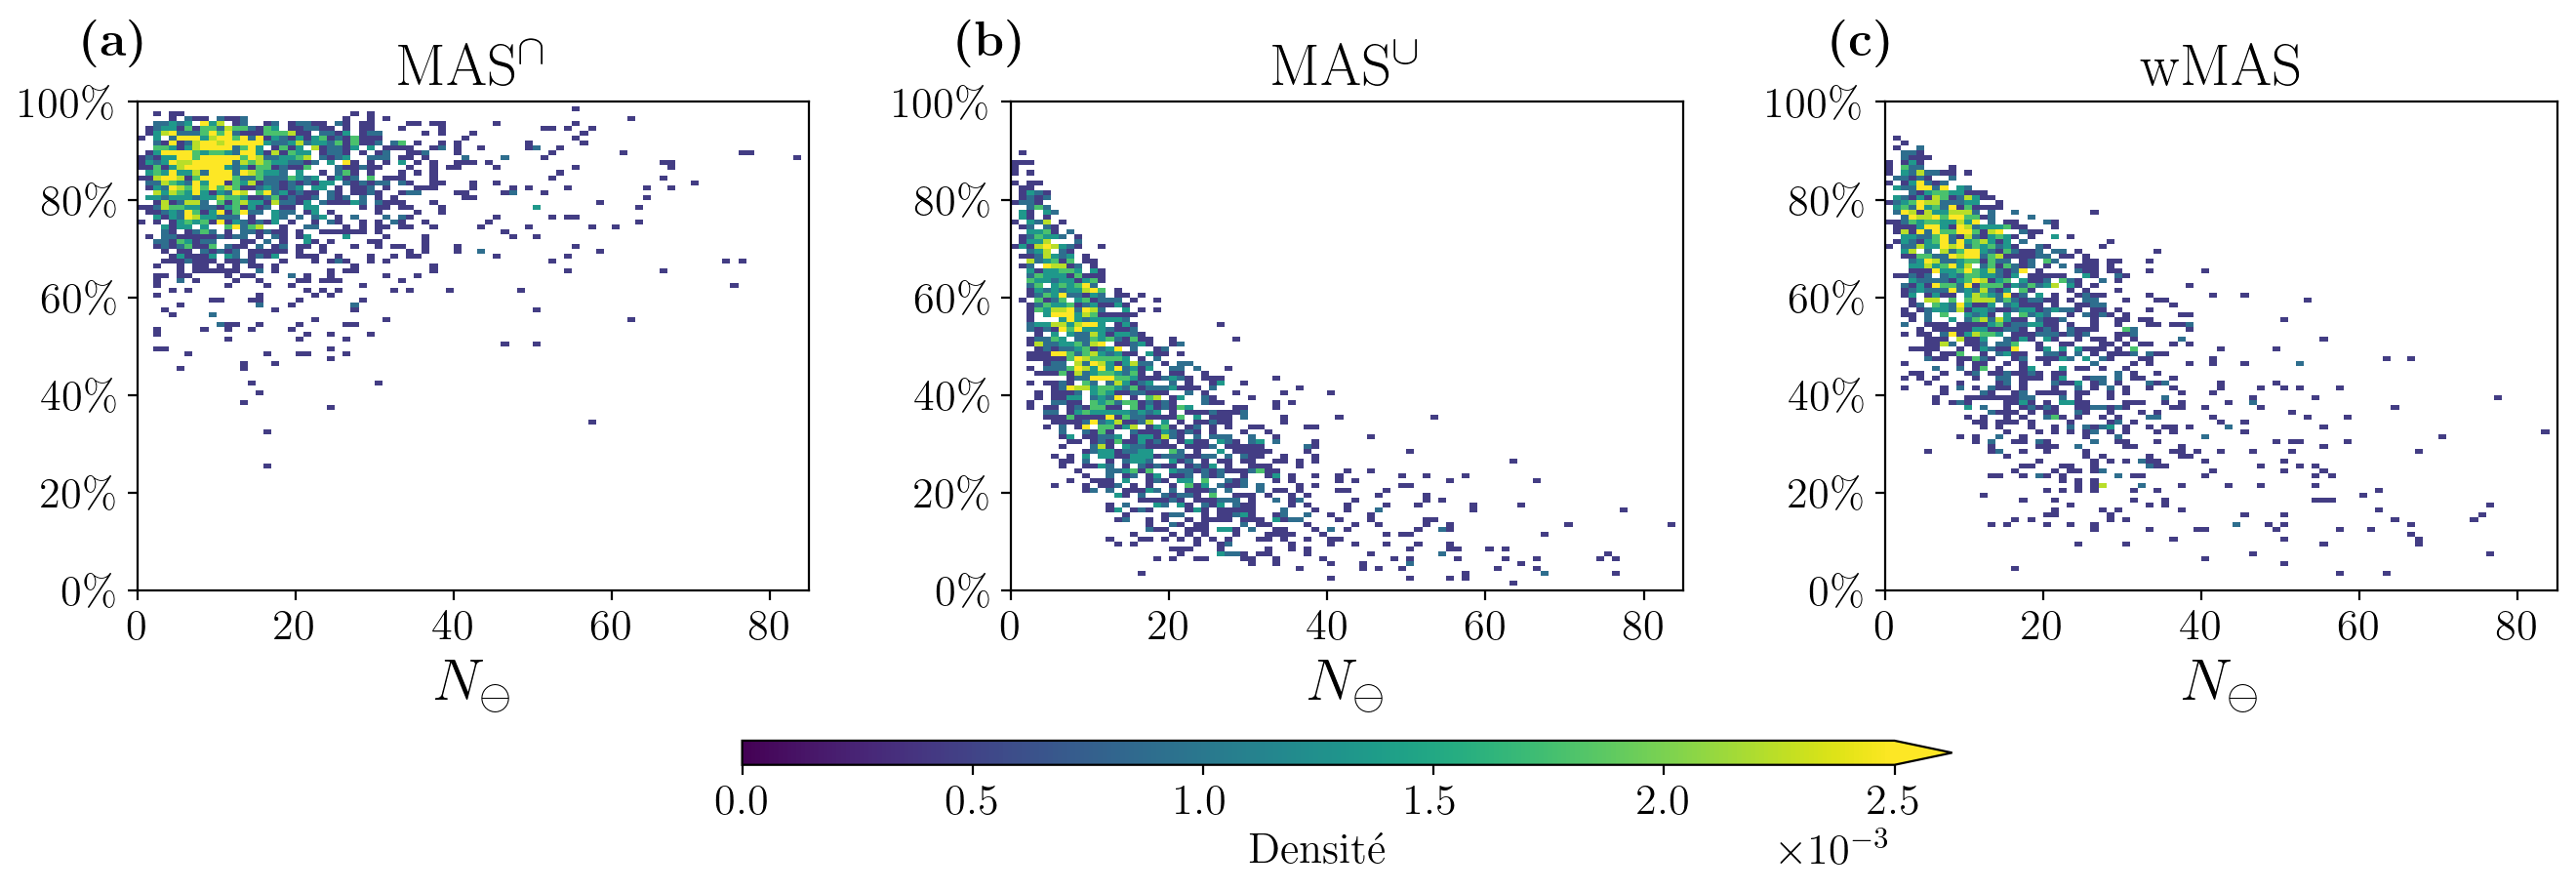
\includegraphics[width=\textwidth]{MAS_vs_Ndiff.png}
    \caption{Caractérisation de la relation entre la similarité des trajectoires en pourcentage et le nombre $N_\ominus$ d'échéances \num{6}-horaires contenu
    dans $C \ominus Q$, pour les trois métriques MAS$^\cap$, MAS$^\cup$ et wMAS de gauche à droite respectivement (a,b et c), évaluées sur \num{2244} paires de
    trajectoires ERA5 / IBTrACS.}
    \label{fig:MAS_Ndiff}
\end{figure}
%
De par sa définition, le MAS$^\cap$ ne dépend que des vecteurs de déplacement sur l'intersection des trajectoires, si bien qu'aucune relation avec $N_\ominus$
ne se dégage. L'encadré (a) met également en évidence une grande similarité angulaire moyenne, avec un MAS$^\cap$ moyen et médian à \prct{83} et \prct{85},
respectivement. La dispersion de ces scores est également très faible, avec un écart type à \prct{9}. Toutefois, la distribution jointe de MAS$^\cap$ montre
également le défaut de cette métrique, puisqu'une similarité évaluée à plus de \prct{80} lorsque $N_\ominus$ est large (jusqu'à $10 N_\cap$) pose question sur
le sens de cette mesure. C'est en réponse à ce constat que le MAS$^\cup$ a été défini, dont la distribution jointe avec $N_\ominus$ est présentée sur la
\cref{fig:MAS_Ndiff}, encadré (b). Pour cette seconde métrique, les scores de similarité sont d'une part diminués, et également largement dispersés. Le
MAS$^\cup$ présente en effet une moyenne et une médiane tous deux à \prct{42} ---~soit près de deux fois moins qu'avec MAS$^\cap$~--- tandis que l'écart-type
est de \prct{18}. En outre, cette métrique présente une relation très marquée avec $N_\ominus$, quasi-linéaire jusqu'à environ $N_\ominus = 20$, au delà de quoi
la similarité apparaît comme légèrement moins sensible à la différence de taille. La différence entre MAS$^\cap$ et MAS$^\cup$ est particulièrement prononcée,
et l'impact de $N_\ominus$ sur MAS$^\cup$ est très fort, à tel point que le problème inverse à celui de MAS$^\cap$ peut se poser, à savoir que la
comptabilisation des échéances sur $C \ominus Q$ avec le même poids que celles sur $C \cap Q$ peut parfois s'avérer très punitive, comme illustré sur les trois
exemples de la \cref{fig:exemple_MAS}. Le wMAS (\cref{fig:MAS_Ndiff} encadré c) vise donc à compenser cette propriété du MAS$^\cup$ via ses coefficients de
pondération qui modifient la contribution de $C \cap Q$ et de $C \ominus Q$ en fonction de la similarité moyenne obtenue sur l'intersection. La distribution du
wMAS est intermédiaire entre MAS$^\cap$ et MAS$^\cup$, avec \prct{59} en moyenne et \prct{62} en valeur médiane. Si on distingue toujours une relation linéaire
entre wMAS et $N_\ominus$, la dispersion des valeurs de $N_\ominus$ autour du score moyen est plus élevée que dans le cas de MAS$^\cup$, indiquant que le wMAS
parvient en effet à compenser des valeurs larges de $N_\ominus$ lorsque $\bar{S_\theta}^\cap$ est élevé. Les exemples de la \cref{fig:exemple_MAS} illustrent ce
point. Ce faisant, le wMAS perd néanmoins en interprétabilité.

\begin{figure}[htbp]
    \centering
    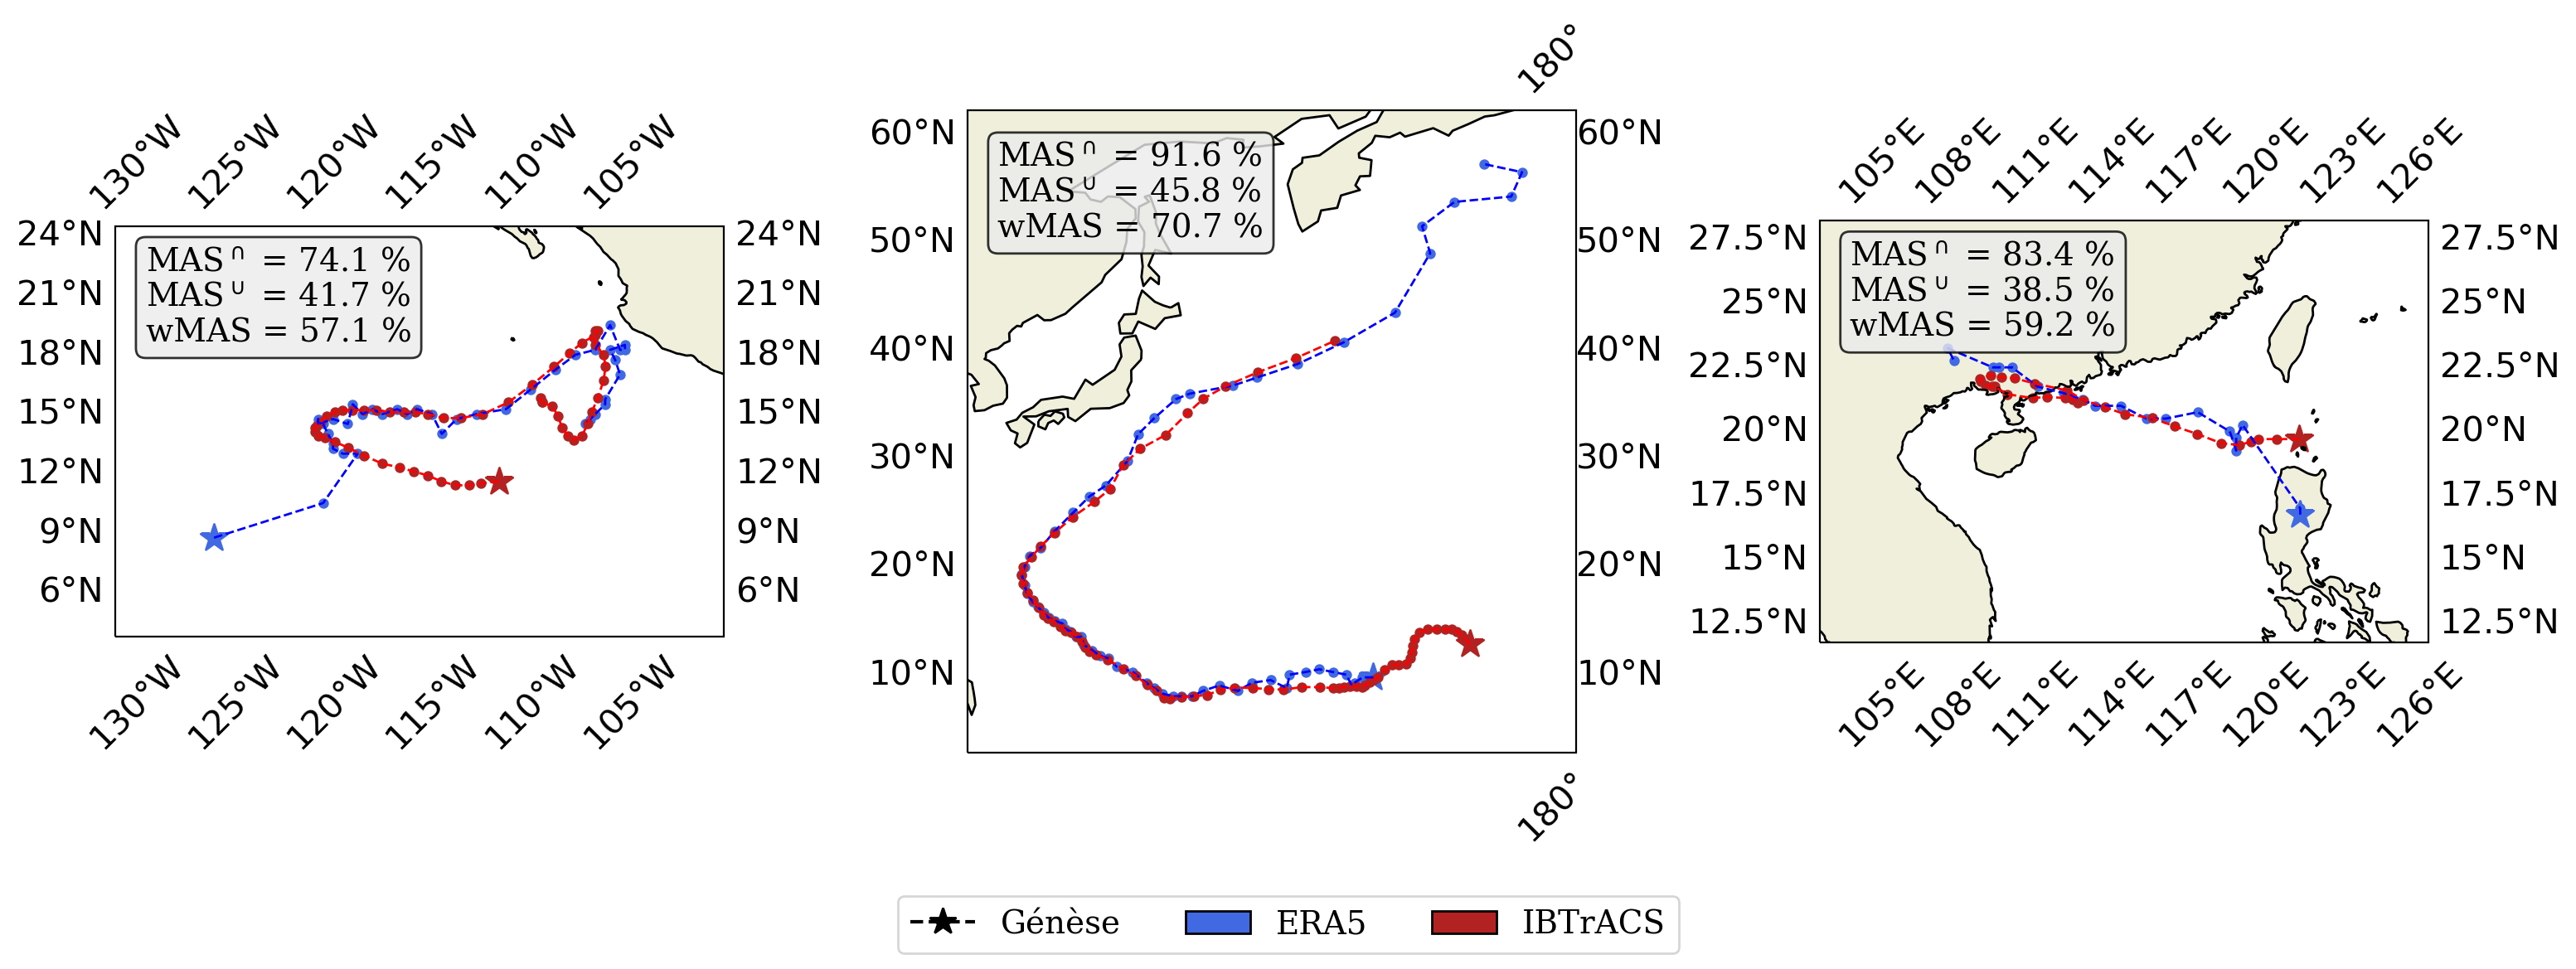
\includegraphics[width=\textwidth]{exemple_MAS_3_tracks.png}
    \caption{Exemple de trois paires de trajectoires sélectionnées parmi les \num{2244}, avec leurs scores de similarité pour chacune des trois métriques
    indiqués dans l'encadré en haut à gauche.}
    \label{fig:exemple_MAS}
\end{figure}

Pour déterminer si l'ajustement des paramètres de détection dont a fait l'objet le traqueur dans le but de maximiser la probabilité de détection a affecté la
similarité des trajectoires, on calcule les valeurs des trois métriques de MAS pour les couples de trajectoires ERA5 / IBTrACS obtenus avant l'optimisation afin
de les comparer aux similarités que les trajectoires actuelles présentent avec ces mêmes trajectoires IBTrACS. Les tracjectoires ERA5 dites
\textquote{non-optimisées} et prises comme référence ici ont été obtenues avec les seuils \textbf{VOR}~$=$~\SI{5e-5}{\per\second}, \textbf{RES}~$=$~\ms{15},
\textbf{TANOM}~$=$~\SI{1}{\kelvin}, \textbf{PT}~$=$~\SI{-2}{\kelvin} et \textbf{PW}~$=$~\ms{5}. Ces valeurs seuils se distinguent de celles utilisées dans
\cite{dulac_assessing_2023} et \cite{bourdin_intercomparison_2022} par la vorticité (respectivement \SI{15e-5}{\per\second}), le seuil de vent (respectivement
\ms{5}) ainsi que le profil vertical de température (respectivement \SI{-1}{\kelvin}). Le paramètre de relaxation est maintenu à \SI{25e-5}{\per\second} entre
les deux jeux de données. La solution non-optimisée présente un POD moyen sur les cinq bassins d'intérêt diminué de plus de \num{10} points de pourcentage,
l'impact le plus prononcé étant sur les bassins NAtl et EPac. Cette diminution du POD se traduit par un déficit de \num{465} couples ERA5 / IBTrACS par rapport
aux trajectoires optimisées, puisque \num{1779} trajectoires ERA5 sont appariées avec les trajectoires de référence. Parmi ces paires de trajectoires,
\num{1649} d'entre elles partagent la même composante IBTrACS, indiquant que \num{130} paires sont manquantes dans les trajectoires dites
\textquote{optimisées}. Cette perte peut s'expliquer par le coût non-négligeable en POD du filtre de systèmes de moyennes latitudes utilisé dans
\cite{dulac_assessing_2023}, filtre non appliqué sur les trajectoires de référence. En effet, le schéma de détection optimisé consiste essentiellement en un
relâchement des contraintes définissant un cyclone tropical, conduisant à un plus grand nombre de systèmes détectés et appariés, notamment des systèmes peu
intenses qui parfois ne présentent pas un cœur chaud suffisamment marqué selon le paramètre $V_U^T$ de \cite{hart_cyclone_2003} sur lequel est fondé le filtre.
Il reste donc \num{1649} cyclones observés dans IBTrACS pour lesquels nous disposons de deux trajectoires ERA5 issues de paramètres de détection différents.
On compare alors la similarité de chacune d'elles évaluée sur le cyclone observé, et pour les trois métriques de similarité présentées précédemment. La première
ligne de la \cref{fig:delta_MAS} présente les distributions de ces changements par rapport aux trajectoires issues du schéma de détection non-optimisé.

\begin{figure}[htb]
    \centering
    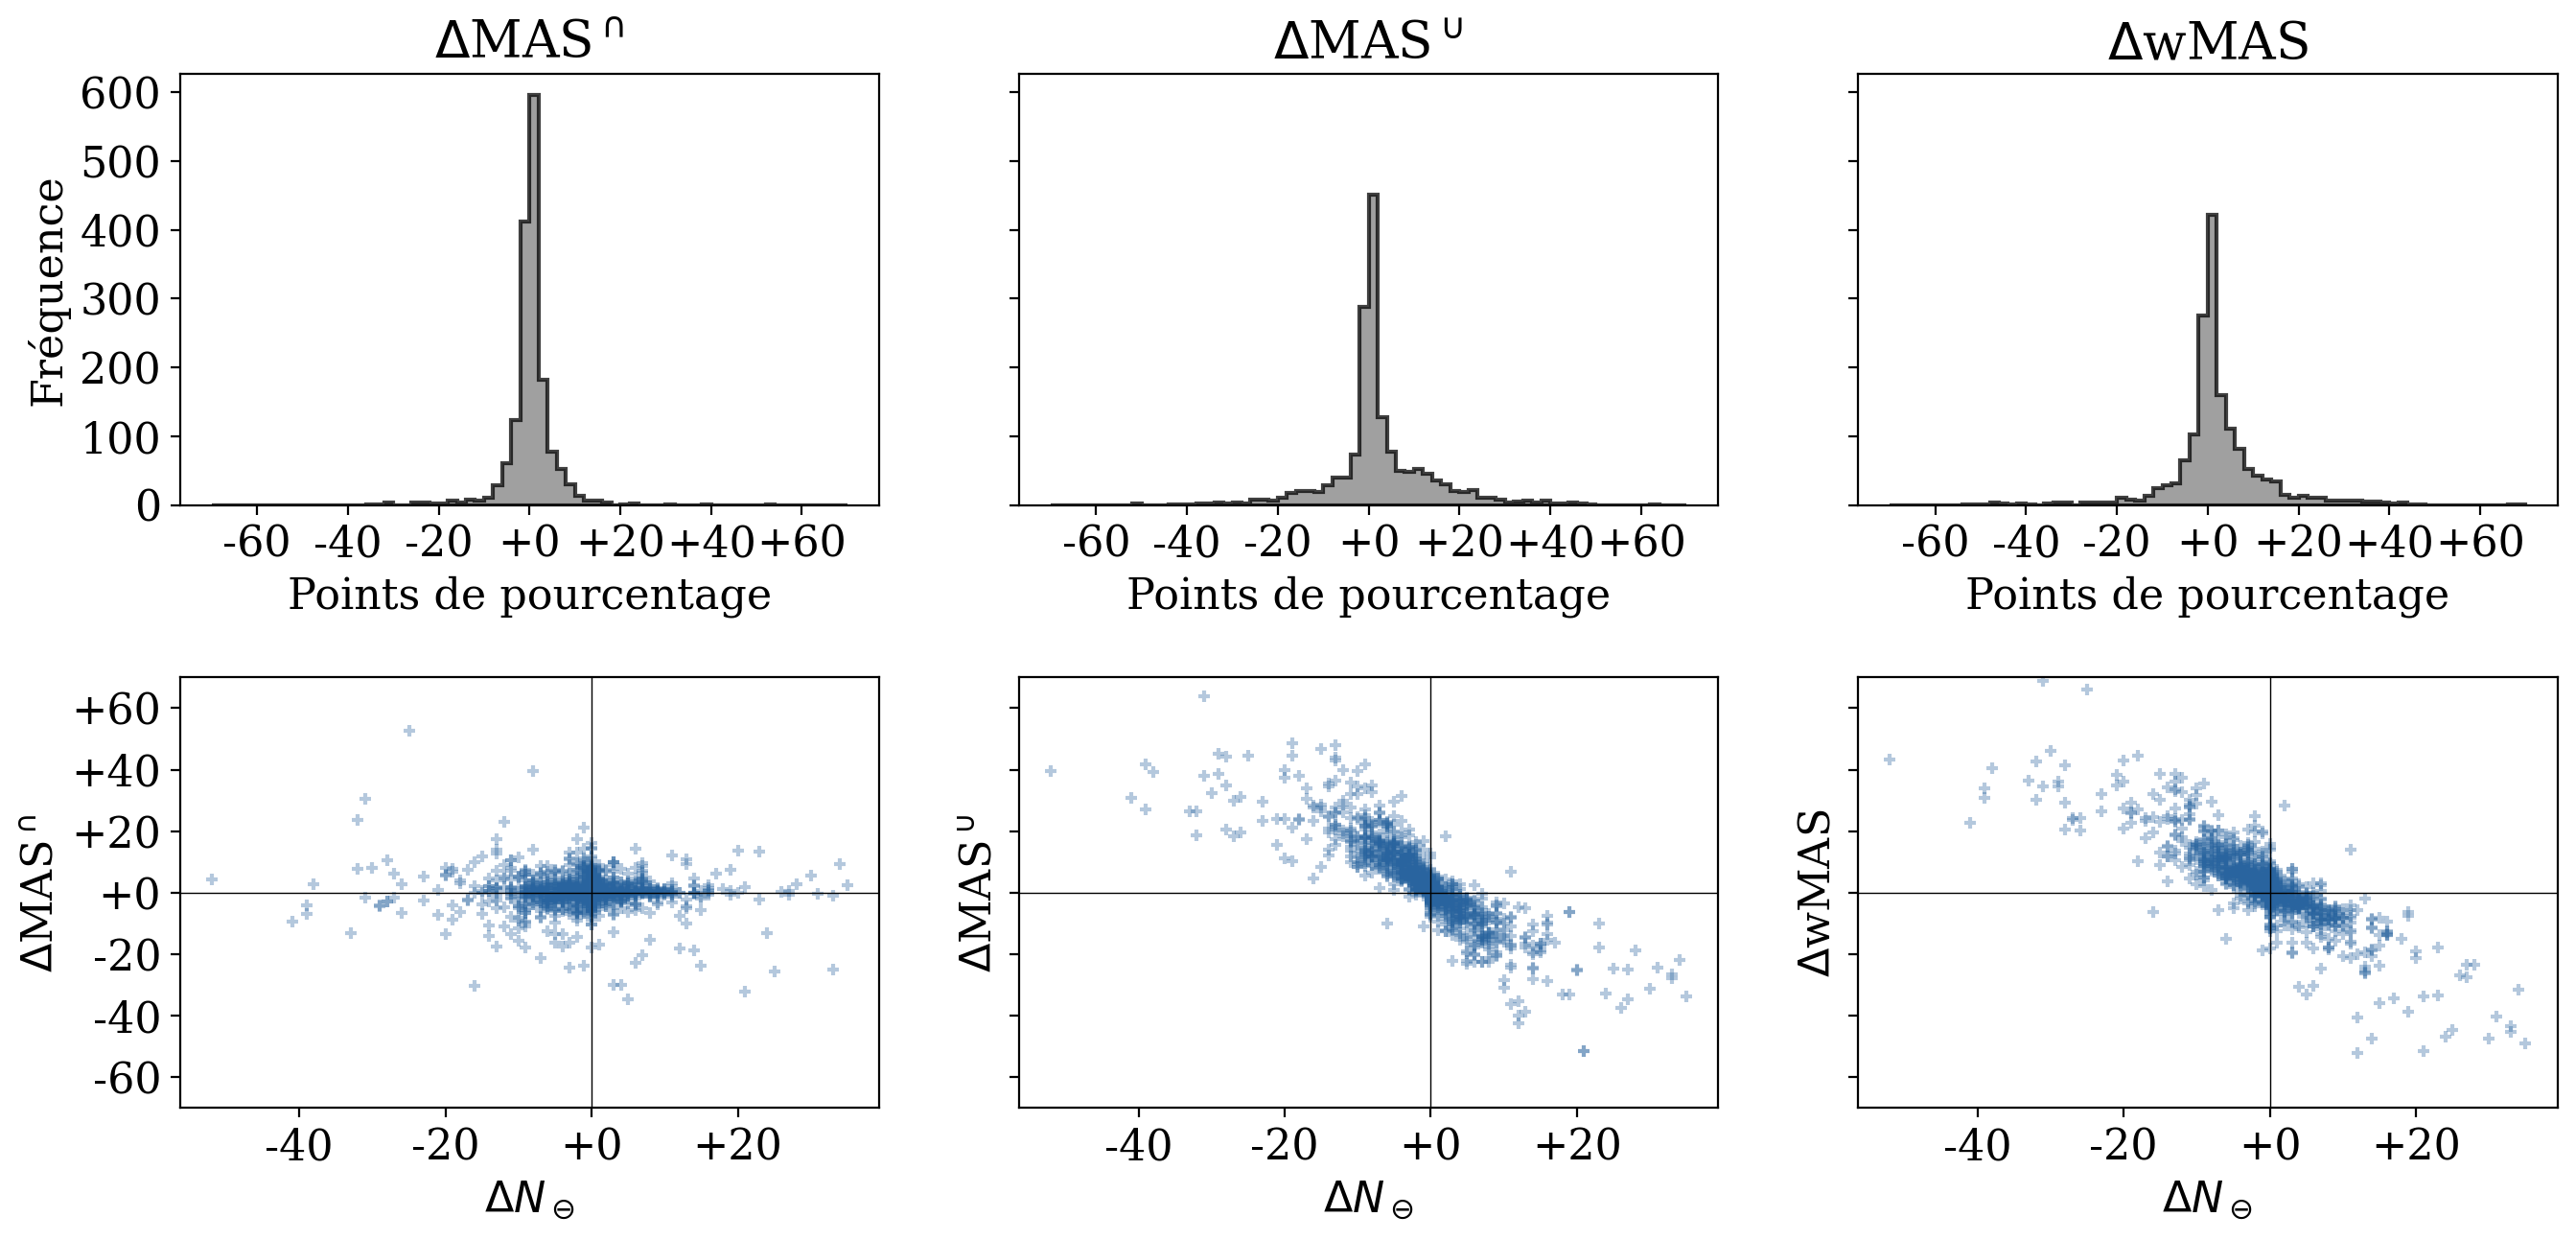
\includegraphics[width=\textwidth]{delta_MAS.png}
    \caption{Distributions du changement dans la similarité des couples de trajectoires ERA5 / IBTrACS (première ligne), par rapport au schéma de détection
    non-optimisé, et pour chacune des trois métriques de similarité (colonnes). Bins de \num{-70} points à \num{70} points avec une largeur de \num{2}
    points. Changement dans la similarité des couples de trajectoires en fonction du changement dans le nombre d'échéances $N_\ominus$ (seconde ligne).}
    \label{fig:delta_MAS}
\end{figure}

Les trois distributions mettent en avant des changements de similarité pour l'essentiel centrés autour de \num{0}. En particulier, la distribution de $\Delta
\text{MAS}^\cap$ présente une moyenne à $+$\num{0.3} points de pourcentage (p.p), et une médiane à $+$\num{0.14} p.p. Si cette moyenne apparaît comme
significativement différente de \num{0} avec test à \prct{95} (valeur-p $=$ \num{0.008}), ce changement est néanmoins insignifiant et peut probablement
s'expliquer par le fait que $N_\cap$ tend à augmenter avec le schéma optimisé ($+$\num{1.9} pas de temps en moyenne), si bien que la similarité angulaire
moyennée sur $C \cap Q$ devient moins sensible aux incohérences locales entre les deux trajectoires. Les deux métriques prenant en considération les échéances
sur $C \ominus Q$ présentent quant à elles une tendance plus claire, bien que toujours faible, vers une amélioration de la similarité, et plus prononcée dans le
cas de MAS$^\cup$ que pour le wMAS. Ces deux distributions indiquent respectivement une moyenne à $+$\num{2.4} p.p et $+$\num{2.05} p.p. Cette évolution est
largement liée au changement de $N_\ominus$ ($-$\num{0.8} pas de temps en moyenne), avec une relation linéaire évidente avec $\Delta N_\ominus$. Un ajustement
linéaire des deux métriques avec $\Delta N_\ominus$ permet d'expliquer \prct{74} de la variance dans le cas de MAS$^\cup$ et \prct{72} dans le cas de wMAS. Mais
cela ne signifie pas pour autant que l'augmentation constatée dans ces deux métriques n'est qu'un artefact. En effet, rappelons que $N_\ominus$ mesure la
différence dans la temporalité des deux trajectoires, si bien que $\Delta N_\ominus < 0$ pour une même trajectoire IBTrACS indique que la trajectoire ERA5 issue
du schéma optimisé présente un début et/ou une fin plus proche de la trajectoire observée. Ainsi, une diminution de $N_\ominus$ avec un MAS$^\cap$ inchangé
constitue en soi une amélioration de la ressemblance des trajectoires. Par ailleurs, il est intéressant de constater sur la seconde ligne de la
\cref{fig:delta_MAS} que, pour les trois métriques considérées, les distributions des changements dans la similarité pour les cas où $\Delta N_\ominus = 0$ sont
faiblement décentrées du côté positif. Précisions toutefois que $\Delta N_\ominus =0$ ne signifie pas nécessairement que les deux trajectoires ERA5 partagent la
même temporalité. Pour s'en convaincre, il suffit de considérer une trajectoire ERA5 qui, dans un jeu de données, ne détecterait pas la dernière échéance de la
trajectoire observée, tandis que la trajectoire équivalente dans le second jeu de données en détecterait une de trop. Une telle situation serait caractérisée
par $\Delta N_\ominus = 0$ et $\Delta N_\cap = +1$. Pour déterminer le changement moyen pour les cas où les deux trajectoires ERA5 sont définies sur exactement
les mêmes dates, il faut donc considérer $\Delta N_\ominus = 0$ et $\Delta N_\cap$ = 0, ce qui correspond à \num{691} cas (\num{721} cas pour la condition
$\Delta N_\ominus = 0$ seule). Le changement moyen de similarité lorsque ces deux conditions sont réunies vaut $+$\num{0.57} p.p, $+$\num{0.34} p.p et
$+$\num{0.54} p.p pour MAS$^\cap$, MAS$^\cup$ et wMAS respectivement. Il semble par conséquent que l'optimisation du schéma de détection de cyclones tropicaux
dans le but de maximiser la probabilité de détection dans ERA5 par rapport à IBTrACS a pu, toutes choses égales par ailleurs, très légèrement améliorer la
similarité des trajectoires détectées avec celles observées, selon la définition de la similarité utilisée ici.

\subsubsection*{Discussion}

En définitive, trois métriques de similarité des trajectoires, toutes basées sur la similarité angulaire $S_\theta$ définie entre deux vecteurs de déplacement
relatif, mais se distinguant par leur prise en charge (ou l'absence) des pas de temps pour lesquels une seule des deux trajectoires existe, sont définis ou
comparés. Étant donné que la similarité de deux trajectoires comporte une part importante de subjectivité, il n'est pas possible de conclure sur les
performances de chacune. Le choix de la métrique dépend en effet de l'usage qui lui est destinée. Le MAS$^\cap$ ne considère que les échéances pour lesquelles
les deux trajectoires coexistent, et peut donc indiquer un excellent score pour des trajectoires pourtant extrêmement différentes. Le MAS$^\cup$ suit la
démarche inverse de compter comme nulle la similarité angulaire sur les échéances où une seule trajectoire existe, si bien qu'une faible différence dans la
taille des trajectoires peut conduire à un score sensiblement diminué. Le wMAS quant à lui, vise à accomplir la tâche pourtant impossible de quantifier avec une
métrique objective une impression subjective de similarité. Si cette approche est par nature vouée à l'échec, le wMAS remplit néanmoins parfaitement son rôle
consistant à nuancer le MAS$^\cup$, se situant ainsi entre les deux autres, et accomplit cela en pondérant les similarités nulles sur $C \ominus Q$ en fonction des
performances sur $C \cap Q$, au détriment de l'interprétabilité de la mesure. Cette caractéristique commune aux trois métriques d'être basées sur une valeur moyenne de
la similarité angulaire présente toutefois l'inconvénient d'être peu sensible aux incohérences locales, ce qui est d'autant plus vrai que les trajectoires sont
longues. En tout état de cause, ces deux catégories de métriques ---~celles basées uniquement sur $C \cap Q$ et celles prenant en considération $C \ominus
Q$~--- ne sont pas à mettre en opposition, car l'usage d'une de chaque peut s'avérer porteur d'informations complémentaires importantes.

Cette analyse visait à déterminer si la recherche des seuils de détection maximisant la probabilité de détection dans la réanalyse ne s'était pas faite au
détriment de la capacité du schéma de détection à fidèlement identifier les trajectoires cycloniques, dans la mesure où la condition implicitement suffisante à
remplir dans la fonction d'objectif que représente le POD dans ce contexte ne consiste qu'à identifier un seul point se trouvant à moins de \km{300} d'une
trajectoire observée. Les résultats de l'étude indiquent que non seulement la similarité n'a, dans l'ensemble, pas diminuée suite à l'optimisation du traqueur,
mais aussi que cette optimisation s'est accompagnée en moyenne d'une amélioration marginale. Cette dernière est en grande partie due au fait que la temporalité
trajectoires détectées par le traqueur optimisé sont souvent plus proches de celles observées que celles issues du traqueur de référence, aussi bien à travers
$N_\ominus$ que $N_\cap$. Cependant, une petite amélioration est visible pour les cas où la longueur est inchangée entre les deux jeux de données. L'analyse
suggère par conséquent que l'impact de l'optimisation du traqueur sur la ressemblance des trajectoires de la réanalyse avec celles observées est au mieux,
marginalement positif, au pire inexistant.

%--------------------------------------
\section{Synthèse}

\end{document}
